\section{Experiments }
\label{sec.exp}

In this section, we first describe the datasets and evaluation settings used in our experiments. We then present a list of research questions we want to address, and accordingly elaborate our experiment results. Finally, we discuss some potential threats to the validity of our approach.

% We then describe our evaluation metrics and experimental settings in Section~\ref{sec:metrics}. Next, we present the research questions in Section~\ref{sec:rqs}. The results of our experiments which answer the research questions are described in Sections~\ref{sec:rq1},~\ref{sec:rq2}~\&~\ref{sec:rq3}. Threats to validity are listed in Section~\ref{sec:threats}

\subsection{Dataset}\label{sec:dataset}

%To evaluate our approach, we use a dataset of 157 bugs from four popular software projects. The four projects are AspectJ~\cite{aspectj_link}, Ant~\cite{ant_link}, Lucene~\cite{lucene_link}, and Rhino~\cite{rhino_link}. All four projects are medium-large scale and implemented in Java. AspectJ, Ant, and Lucene contain more than 300 kLOC, while Rhino contains almost 100 kLOC. {\iffalse \color{red} (Duy: AspectJ uses BugZilla )These four projects use Jira as the issue tracking system, from which we retrieve their bug reports. Bissyande et al. found that in Jira bugs are generally well linked to commits that fix them~\cite{BissyandeTWLJR13}.\fi} Table~\ref{tab:dataset} describes detailed information of the four projects in our study.

To evaluate our approach, we use a dataset of 355 bugs from seven popular software projects. The seven projects are Ant~\cite{ant_link}, AspectJ~\cite{aspectj_link}, Lang~\cite{lang_link}, Lucene~\cite{lucene_link}, Math~\cite{math_link}, Rhino~\cite{rhino_link}, and Time~\cite{time_link}. All seven projects are medium-large scale and implemented in Java. Ant, AspectJ, and Lucene contain more than 300 kLOC. Math, Rhino, and Time contains almost 100 kLOC, while Lang only contains more than 50 KLOC. Ant, AspectJ, Lang, Lucene, Math, and Rhino projects use Jira as the issue tracking system, from which we retrieve their bug reports. Bissyande et al. found that in Jira bugs are generally well linked to commits that fix them~\cite{BissyandeTWLJR13}. Time uses Github as the issues tracking system, from which we collect their bug reports. Table~\ref{tab:dataset} describes detailed information of the seven projects in our study.

%
%\begin{table*}[t]
%	\center
%	\caption{Dataset Description}
%    \begin{tabular}{|c|c|c|c|c|c|c|c|c|c|c|c|}
%    \hline	
%     \multirow{2}{*}{\textbf{Project}}& \textbf{Number of}  &\multirow{2}{*}{\textbf{Study Perid}} & \multicolumn{3}{c|}{\textbf{Number of Methods}} & \multicolumn{3}{c|}{\textbf{Number of Failed Testcases}}  & \multicolumn{3}{c|}{\textbf{Number of Passed Testcases}}\\\cline{4-12}
%         ~ & \textbf{Bug Reports} & ~ & \textbf{Max} & \textbf{Median} & \textbf{Min} &\textbf{Max} & \textbf{Median} & \textbf{Min} & \textbf{Max} & \textbf{Median} & \textbf{Min} \\
%     \hline\hline
%    AspectJ & 41 & Mar. 2005 - Feb. 2007 & 28,083 & 13,908 & 10,683 & 9 & 1 & 1 & 818 & 803 & 52 \\\hline
%    Ant & 53 &  Dec. 2001 - Sept. 2013&10,451 &  9,655 & 8,345 &  8 & 1 & 1 & 1,554 & 1,237 & 575 \\\hline
%    Lucene & 37 & June 2006 - Jan. 2011 & 15,487 & 9,416 & 9,103 & 15 & 1 & 1 & 1,160 & 1,090 & 655 \\\hline
%	Rhino & 26 & Dec. 2007 - Dec. 2011 & 5,312 & 4,849 & 3,754 & 7 & 1 & 1 & 185~ & 104.5 & 111 \\\hline
%
%    \end{tabular}
%    \label{tab:dataset}
%\end{table*}

\begin{table}[t]
	\centering
	\caption{Dataset Description}
	%\scalebox{0.92}{
    \begin{tabular}{|l|c|c|r|}
    \hline
   \multirow{2}{*}{\textbf{Project}} &\multirow{2}{*}{\textbf{\#Bugs}}&{\multirow{2}{*}{\textbf{Time Period}}}& \textbf{Average}   \\
    ~       &             &                                   &\textbf{\# Methods}   \\ \hline
	\hline
	Ant       & 53                                          & 12/2001 -- 09/2013 & 9,624.66   \\ 
    AspectJ       & 41                                              & 03/2005 -- 02/2007                                   & 14,218.39   \\ 
%    \hline
     
%     \hline
Lang       &     65                                          & 	10/2002 -- 	04/2016 & 2,151.1  \\
    Lucene       & 37                                              & 06/2006 -- 01/2011                   & 10,220.14   \\
    Math       & 106                                              &  12/2004 --  03/2016& 4,792.3   \\ 
%    \hline
    Rhino       & 26                                                 &  12/2007 -- 12/2011                                   & 4,839.58   \\
    Time       & 27                                                 &                      05/2004 -- 03/2017            & 4,083.5
    \\ \hline
    \end{tabular}
    %}
    \label{tab:dataset}
\end{table}

%The 41 AspectJ bugs are from the iBugs dataset which was collected by Dallmeier and Zimmermann~\cite{DallmeierZ07}. Each bug in the iBugs dataset comes with the code before the fix (pre-fix version), the code after the fix (post-fix version), and a set of test cases. The iBugs dataset contains more than 41 AspectJ bugs, but not all of them come with failing test cases. Test cases provided in the iBugs dataset are obtained from the various versions of the regression test suite that comes with AspectJ. The remaining 116 bugs from Ant, Lucene, and Rhino were collected by ourselves, following the procedure used by Dallmeier and Zimmermann~\cite{DallmeierZ07}. For each bug, we collected the pre-fix version, post-fix version, a set of successful test cases, and at least one failing test case. A failing test case is often included as an attachment to a bug report or committed along with the fix in the post-fix version. When a developer receives a bug report, he/she first needs to replicate the error described in the report~\cite{worksforme}. In this process, he is creating a failing test case. Unfortunately, not all test cases are documented and saved in the version control systems.

The 116 bugs from Ant, Lucene, and Rhino were collected by ourselves, following the procedure used by Dallmeier and Zimmermann~\cite{DallmeierZ07}. For each bug, we collected the pre-fix version, post-fix version, a set of successful test cases, and at least one failing test case. A failing test case is often included as an attachment to a bug report or committed along with the fix in the post-fix version. When a developer receives a bug report, he/she first needs to replicate the error described in the report~\cite{worksforme}. In this process, he is creating a failing test case. Unfortunately, not all test cases are documented and saved in the version control systems. The 41 AspectJ bugs are from the iBugs dataset which was collected by Dallmeier and Zimmermann~\cite{DallmeierZ07}. Each bug in the iBugs dataset comes with the code before the fix (pre-fix version), the code after the fix (post-fix version), and a set of test cases. The iBugs dataset contains more than 41 AspectJ bugs, but not all of them come with failing test cases. Test cases provided in the iBugs dataset are obtained from the various versions of the regression test suite that comes with AspectJ. We collected the remaining 198 bugs from Lang, Math, and Time from Defects4J benchmark~\cite{Just:2014:DDE:2610384.2628055}, a database of real, isolated, reproducible software faults from real-world open-source Java projects. The three projects include a large number of test cases, and there exists at least one failing test case per bug. 
%We note that Math originally has 106 bugs. However, there are three bugs that we are unable to find their bug reports, and hence we omit these three bugs. For this reason, Math only contains 103 bugs. 


%By doing this, the developer is actually creating a system test case that fails in the pre-fix version but will pass in the post-fix version.

%\begin{table}[t]
%	\centering
%	\caption{Statistics of Collected Traces}
%    \begin{tabular}{|l||r|r|r||r|r|r|}
%    \hline
%    \multirow{2}{*}{\text{Project}} & \multicolumn{3}{c||}{\text{Failed Traces}}  & %\multicolumn{3}{c|}{\text{Passed Traces}}   \\ \cline{2-7}
%    ~ & Min & Median & Max & Min & Median & Max  \\ \hline
%	\hline
%Ant&1&2.0&8&575&1212.0&1554\\\hline
%AspectJ&1&1.0&9&52&802.0&818\\\hline
%Lucene&1&1.0&15&655&1076.0&1160\\\hline
%Rhino&1&1.0&7&11&101.5&185\\\hline


%    \end{tabular}
%    \label{tab:traces_statistics}
%\end{table}
%Since multi-modal bug localization techniques require both textual information in bug reports and program spectra, we select bug reports whose failing test cases are available.

%{\color{red} These three projects use Jira as the issue tracking system, from which we retrieve their bug reports. Bissyande et al. found that in Jira bugs are generally well linked to commits that fix them~\cite{BissyandeTWLJR13}.}
%{\iffalse We analyzed all bug reports of Ant from version 1.5.1 to 1.9.2, Lucene from version 2.0 to 3.1, and Rhino from version 1.6 to 1.7 and find those whose failing test cases are available.\fi}
%{\color{red} Table~\ref{tab:dataset} describes study periods of the three projects.}

%The Among 157 bugs, we use 41 bugs of AspectJ from iBugs dataset\footnote{http://www.st.cs.uni-saarland.de/ibugs/}. For the remaining 116 bugs, we manually collect Ant, Lucene, and Rhino's repositories.
%From the four projects, we have 157 bugs that we are able to find at least one test case that is failed in the before-fix version, and passed in the after-fix version.

%AspectJ, Ant, Lucene, Rhino
%AspectJ: ibugs
%why choose these projects ? popular, well documented as fixes are labelled with bug id
%Ant, Lucene, Rhino: manually extract from the repository
%All projects are in Java
%Bug report extract from bug tracking system
%Test cases: failed test case that failed in prefix, and passed in postfix


%We manually finds bugs of Ant, Lucene, and Rhino which have test cases to reproduce the bugs in the faulty programs. Such these test cases are usually attached with bug reports by users, or created by developers during bug-fixing process. From the change history of the projects, we identify the links from bugs to commits as developers usually put bug IDs with commits that have the bug fixes. We select program versions in the the commits right before the linked commits that have the bug fixes as the faulty program versions. Furthermore, we select the bugs whose bug fixes come with test cases. Usually a Junit test case file has name starts or ends ``Test''. Using this heuristic, we select these such bugs, and run the found test cases with before-fix version, and after-fix version of the bug. If the before-fix version returns an unexpected result, and the after-fix version outputs an expected result. We include the bug into our dataset.

%Tablet~\ref{tab:dataset} depicts information of the dataset.
%how to find link from bug to commit
%how to find test case
%after identify the links, and failed test case -> collect data
%for bug: textual bug report ( long description + short description ) + test cases ( failed + passed tests) + source code of prefix + groundtruth methods.

%files in our dataset. Therefore, the amount of effort to inspect  top-10 program methods is equivalent to the amount of effort to examine one single source code file.

\subsection{Evaluation Metrics and Settings}
\label{sec:metrics}

To assess the effectiveness of a bug localization method, we employ two key metrics, namely: Top N and mean average precision (MAP). They are respectively described below:

\begin{itemize}
	\item  \textbf{Top N}: Given a bug report, if one of its corresponding faulty methods is in the top-N results, we consider that the bug is successfully localized. The Top N score of a bug localization method is the number of bugs it can successfully localize~\cite{Zhou:2012:BFM:2337223.2337226,SahaLKP13}.
	\item  \textbf{Mean Average Precision (MAP)}: MAP is an IR metric to evaluate ranking approaches~\cite{Manning2008}, and is computed by taking the mean of the {\em average precision} scores across all bug reports. The average precision of a single bug report is computed as:
	\[
	AP = \frac{\sum_{k=1}^{M}P(k) \times pos(k)}{\sum_{k=1}^{M} pos(k)}
	\]
	where $k$ is a rank in the returned ranked methods, $M$ is the number of ranked methods, and $pos(k)$ indicates whether the $k^{th}$ method is faulty or not. Here $P(k)$ is the precision at a given top $k$ methods, which is computed as follows:
	\[
	P(k)=\frac{\#faulty\ methods\ in\ the\ top\ k}{k}.
	\]
Note that the MAP scores of existing bug localization methods are typically low~\cite{Rao:2011:RSL:1985441.1985451,Sisman:2012:IVH:2664446.2664454,Zhou:2012:BFM:2337223.2337226,SahaLKP13}.
\end{itemize}


%\begin{table}
%	\caption{Experimental Configuration of Algorithm~\ref{alg:adaptive}. $\eta$ = Learning Rate. $\lambda$= Regularization. $T_{max}$ = Maximum of number iteration.}
%	\centering
%    \begin{tabular}{|l|c|c|c|}
%    \hline
%    \textbf{Project} &  $\eta$ &  $\lambda$& $T_{max}$ \\ \hline
%    \hline
%    AspectJ & $10^{-2}$             & $10^{-5}$              & 30     \\ \hline
%    Ant     & $10^{-2}$              & $10^{-5}$               & 30     \\ \hline
%    Lucene  & $10^{-2}$              & $10^{-5}$               &30    \\ \hline
%    Rhino   & $10^{-3}$              &$10^{-3}$               & 30     \\ \hline
%    \end{tabular}
%    \label{tab:configeration}
%\end{table}

%\vspace{0.1cm} {We perform standard 10 fold cross validation (CV) to evaluate our approach. For each project, we divide the bugs into ten sets. We use 9 sets as training data and 1 as testing data. We repeat the process 10 times using different training and testing data combinations. We then aggregate the results to get the final Top N and MAP scores. For our experiments, the learning rate $\eta$ and regularization parameter $\lambda$ of AML are chosen by performing another cross validation on the training data, while the maximum number of iterations $T_{max}$ is fixed as $30$. We also use $K=10$ as default value for the number of nearest neighbors. We conduct experiments on an Intel(R) Xeon E5-2667 2.9GHz server running Linux 2.6.

Our evaluation procedure is based on 10-fold \emph{cross validation} (CV). That is, for each project, we divide the bug reports into ten (mutually exclusive) sets. Then, for each fold, we take 1 set as new bug report queries (i.e., testing set) and treat the remaining 9 sets as historical bug reports (i.e., training set). We repeat this 10 times, and then collate the results to get the aggregated Top N and MAP scores.
	
In all our experiments, the hyper-parameters of the NetML method were configured as follows. Firstly, the regularization parameters $\alpha$ and $\beta$ were chosen by performing 10 fold cross validation on the training set. Next, the maximum number of iterations $T_{max}$ was fixed to $30$. We use $K=10$ as default value for the number of nearest neighbors. Note that the NetML parameters $K$ and $T_{max}$ follow the settings used in AML~\cite{Le:2015:IRS:2786805.2786880}, so as to ensure fair comparisons. All experiments were conducted on an Intel(R) Xeon 2.9GHz server running a Linux operating system.

In order to assess whether NetML substantially outperforms other bug localization methods, we apply \emph{Wilcoxon signed-rank test}~\cite{Wilcoxon1945}; it is a non-parametric statistical significance test for comparing two related or matched samples, whereby the population cannot be assumed to be normally distributed. The Wilcoxon test was applied to two types of metric (i.e., TopN and MAP). For every evaluation metric, we collated the 10-fold results of a bug localization technique across the four software projects (i.e., AspectJ, Ant, Lucene, and Rhino) and then performed the Wilcoxon test to compare the collated results of different techniques. For this test, our null hypothesis is that NetML performs \emph{worse} than or \emph{equal} to the other method, and so we used one-sided/tail $p$-value to validate this hypothesis. Moreover, we also apply the Benjamini-Hochberg (BH)~\cite{Benjamini1995thecontrol} procedure to control the effect of multiple comparisons. If the $p$-value is sufficiently small (say, below a significance level of $0.05$), we can confidently reject the null hypothesis and conclude that NetML is significantly better than the other method.

\subsection{Research Questions}
\label{sec:rqs}

Our empirical study seeks to answer several research questions (RQ), as described in the following subsections.

\subsubsection{RQ1: How Effective is NetML Compared to Other State-of-the-Art Techniques?}

%We compare our NetML approach with its predecessor, i.e., AML~\cite{Le:2015:IRS:2786805.2786880}, and several other state-of-the-art techniques. Previously, PROMESIR~\cite{PoshyvanykGMAR07}, SITIR~\cite{LiuMPR07}, and several variants developed by Dit et al.~\cite{DitRP13} were state-of-the-art multi-modal feature location techniques. Among the variants proposed by Dit et al.~\cite{DitRP13}, the best performing ones were $IR_{LSI}Dyn_{bin}WM_{HITS}(h,bin)^{bottom}$ and  $IR_{LSI}Dyn_{bin}WM_{HITS}(h,freq)^{bottom}$. In this paper, we refer to these variants as DIT$^\text{A}$ and DIT$^\text{B}$ respectively. Dit et al. had shown that these two variants outperform SITIR, and so we exclude SITIR from our study. We also compare NetML with a state-of-the-art IR-based bug localization method named LR~\cite{YeBL14}, and a state-of-the-art spectrum-based bug localization method named MULTRIC~\cite{XuanM14}. Note that, unlike PROMESIR, DIT$^{A}$, DIT$^{B}$, and MULTRIC which locate buggy methods, LR locates buggy files. Thus, we convert the list of files that LR produces into a list of methods by using two heuristics: (1) to return methods in a file in the same order that they appear in the file; and (2) to return methods based on their similarity to the input bug report as computed using a VSM model. We refer to the two variants of LR as LR$^{A}$ and LR$^{B}$ respectively.

We compare out NetML approach with its predecessor, i.e., AML~\cite{Le:2015:IRS:2786805.2786880}, and several other state-of-the-art techniques. Previously, Le et al. proposed SAVANT~\cite{B.Le:2016:LBF:2931037.2931049}, a state-of-the-art fault localization approach that employs a learning-to-rank~\cite{svmrank} strategy, using likely invariant \textit{diffs} and suspiciousness scores as features. OCHIAI~\cite{Abreu:2007:ASF:1308173.1308264} and DSTAR~\cite{DBLP:journals/tr/WongDGL14} are the well-known statistical formula to detect suspicious locations for fault localization without requiring any prior information on program structure or semantics. PROMESIR~\cite{PoshyvanykGMAR07}, SITIR~\cite{LiuMPR07}, and several variants developed by Dit et al.~\cite{DitRP13} were state-of-the-art multi-modal feature location techniques. Among the variants proposed by Dit et al.~\cite{DitRP13}, the best performing ones were $IR_{LSI}Dyn_{bin}WM_{HITS}(h,bin)^{bottom}$ and  $IR_{LSI}Dyn_{bin}WM_{HITS}(h,freq)^{bottom}$. In this paper, we refer to these variants as DIT$^\text{A}$ and DIT$^\text{B}$ respectively. Dit et al. had shown that these two variants outperform SITIR, and so we exclude SITIR from our study. We also compare NetML with a state-of-the-art IR-based bug localization method named LR~\cite{YeBL14}, and a state-of-the-art spectrum-based bug localization method named MULTRIC~\cite{XuanM14}. Note that, unlike PROMESIR, DIT$^{A}$, DIT$^{B}$, and MULTRIC which locate buggy methods, LR locates buggy files. Thus, we convert the list of files that LR produces into a list of methods by using two heuristics: (1) to return methods in a file in the same order that they appear in the file; and (2) to return methods based on their similarity to the input bug report as computed using a VSM model. We refer to the two variants of LR as LR$^{A}$ and LR$^{B}$ respectively.

%measure the suspiciousness of program units based on the execution traces in spectrum-based fault localization. 

For all the above-mentioned techniques, we used the same parameters and settings as described in the respective papers, with the following exceptions that we justify. For DIT$^\text{A}$ and DIT$^\text{B}$, the threshold used to filter methods using HITS was decided ``such that at least one gold set method remained in the results for 66\% of the [bugs]''~\cite{DitRP13}. In this paper, since we used 10-fold CV, rather than using 66\% of all bugs, we used all bugs in the training data (i.e., 90\% of all bugs) to tune the threshold. For PROMESIR, we also used 10-fold CV and applied a brute force approach to tune PROMESIR's component weights using a step of 0.05.

%We first compare NetML against our original multi-modal technique (i.e., AML)~\cite{Le:2015:IRS:2786805.2786880}. AML tries to estimate the method suspiciousness score by computing separate latent parameters for each bug report, and hence allows us to localize bugs more effectively. In this paper, bug localization is considered as ranking of query results problem in information retrieval. In particular, we look at the description of the bug report as a query, and methods as documents. Hence, NetML and AML are employed to sort the methods based on their relevance with the bug reports.  

%In the past, PROMESIR~\cite{PoshyvanykGMAR07}, SITIR~\cite{LiuMPR07}, and several algorithm variants proposed by Dit et al.~\cite{DitRP13} were state-of-the-art multi-modal feature location techniques. Among the variants proposed by Dit et al.~\cite{DitRP13}, the best performing ones were $IR_{LSI}Dyn_{bin}WM_{HITS}(h,bin)^{bottom}$ and  $IR_{LSI}Dyn_{bin}WM_{HITS}(h,freq)^{bottom}$. We refer to them as DIT$^\text{A}$ and DIT$^\text{B}$ in this paper. Dit et al. have shown that these two variants outperform SITIR. 
%However, Dit et al.'s variants have never been compared with PROMESIR. PROMESIR has also never been compared with SITIR. Thus, to answer this research question, we compare the performance of our approach with PROMESIR, DIT$^\text{A}$ and DIT$^\text{B}$.  
%Additionally, the two variants of LR~\cite{YeBL14} (LR$^A$ and LR$^B$) and MULTRIC~\cite{XuanM14} which are recently proposed state-of-the-art IR-based and spectrum-based bug localization techniques respectively. In this paper, we compare NetML against these state-of-the-art techniques, including AML, to evaluate the effectiveness of our proposed approach (i.e., NetML) in bug localization.

\subsubsection{RQ2: Do Feature Components of NetML Contribute toward Its Overall Performance?}

%How effective is AML as compared to different combinations of its components (i.e., $\text{AML}^\text{Text}$, $\text{AML}^\text{Spectra}$, and $\text{AML}^\text{SuspWord}$)

To answer this question, we conducted an ablation test by dropping one feature component (i.e., $\text{NetML}^\text{Text}$, $\text{NetML}^\text{SuspWord}$, or $\text{NetML}^\text{Spectra}$) one-at-a-time and evaluating the performance. In the process, we created three variants of NetML: $\text{All}^{-\text{Text}}$, $\text{All}^{-\text{SuspWord}}$ , and  $\text{All}^{-\text{Spectra}}$. That is, we excluded Text, SuspWord, and Spectra from all feature components, respectively (see also Fig. \ref{fig:framework}). We used the default value of $K=10$, and applied the NetML adaptive learning procedure (i.e., Algorithm \ref{alg:network_lasso}) to tune the latent parameters of these variants. As our baseline, we performed the same ablation test to the feature components of the AML method (i.e., $\text{AML}^\text{Text}$, $\text{AML}^\text{SuspWord}$, or $\text{AML}^\text{Spectra}$).

%To answer this research question, we simply drop one component (i.e., $\text{AML}^\text{Text}$, $\text{AML}^\text{SuspWord}$, and  $\text{AML}^\text{Spectra}$) from AML one-at-a-time and evaluate their performance. In the process, we create three variants of AML: $\text{AML}^{-\text{Text}}$, $\text{AML}^{-\text{SuspWord}}$ , and  $\text{AML}^{-\text{Spectra}}$. To create $\text{AML}^{-\text{Text}}$, $\text{AML}^{-\text{SuspWord}}$ , and  $\text{AML}^{-\text{Spectra}}$, we exclude $\text{AML}^{\text{Text}}$, $\text{AML}^{\text{SuspWord}}$ , and  $\text{AML}^{\text{Spectra}}$ components from Equation~\ref{eqn:composite} of our proposed AML, respectively. We use the default value of $K=10$, and apply Algorithm~\ref{alg:adaptive} to tune weights of these variants, and compare their performance with our proposed AML.

%question investigate the performance of different combinations of three AML components . In total, we compare 6 variants of AML with our proposed AML (Section~\ref{subsec:adaptive}). These variants are $\text{AML}^\text{Text}$, $\text{AML}^\text{SuspWord}$,  $\text{AML}^\text{Spectra}$, .

%By excluding one component from Equation~\ref{eqn:composite}, we formulate three different variants of AML. They are $\text{AML}^{-\text{Text}}$, $\text{AML}^{-\text{SuspWord}}$, and $\text{AML}^{-\text{Spectra}}$. In $\text{AML}^{-\text{Text}}$, we exclude $\text{AML}^\text{Text}$ component from Equation~\ref{eqn:composite}. Similarly, we remove $\text{AML}^\text{SuspWord}$, and  $\text{AML}^\text{Spectra}$ from Equation~\ref{eqn:composite} to create $\text{AML}^{-\text{SuspWord}}$, and  $\text{AML}^{-\text{Spectra}}$, respectively. We also investigate performance of each component when they are isolated.

%To answer this question, we use the default value of $n=10$, and apply Algorithm~\ref{alg:adaptive} to tune weights of the three variants for bug localization. Then, we compare the performance  of the three variants with the original AML in term of Mean Average Precision.

\subsubsection{RQ3: How Effective is the NetML Integrator?}

Instead of using the NetML integrator component (see Section \ref{sec.generalized_adaptive}), one may consider using a standard machine learning algorithm, such as the learning-to-rank method, to combine the scores produced by the three feature components. Indeed, state-of-the-art IR-based and spectrum-based bug localization techniques such as LR and MULTRIC are based on the learning-to-rank method. As such, we conduct an experiment to compare our NetML integrator model with an off-the-shelf learning-to-rank model called SVM$^{rank}$~\cite{svmrank}, which was also used by LR~\cite{YeBL14}. To do so, we simply replace the NetML integrator model in Fig. \ref{fig:framework} with SVM$^{rank}$, and then compare the resulting performances. For completeness, we also compare our NetML integrator with the integrator model used by the AML algorithm.

\newcolumntype{C}[1]{>{\centering\arraybackslash}p{#1}}
\newcolumntype{L}[1]{>{\raggedright\arraybackslash}p{#1}}



%\noindent
%\textbf{Research Question 4:} How efficient is AML?
%
% If AML takes hours to produce a ranked list of methods for a given bug report, then it would be less useful. In this research question, we investigate the average running time needed for AML to output a ranked list of methods for a given bug report.



\subsubsection{RQ4: What is the Effect of Varying the Number of Neighbors $K$ on the Performance of NetML?}

The most important parameter in our NetML approach is the number of nearest neighbors $K$ (while the regularization parameters $\alpha$ and $\beta$ were chosen via cross-validation---see Section \ref{sec:metrics}). By default, we set the number of neighbors to $K=10$, but the effect of varying this value is unclear. To answer this research question, we vary the value of $K$ and investigate its effects on the performance of NetML. In particular, we wish to investigate if the performance remains relatively stable with varying values of $K$. For each $K$ value, we also compare the performance of NetML against its predecessor (i.e., AML) using the same value.

%\vspace{0.2cm}\noindent
%\textbf{Research Question 5:} Which of the three components of AML contributes the most to the effectiveness of AML?

%\vspace{0.2cm} AML has three components AML$^\text{Text}$, AML$^{\text{Spectra}}$, and AML$^{SuspWord}$ that assign scores to methods. For each individual bug, the adaptive integrator component of AML learns weights that govern the contribution of these three components. It is unclear which of the three components contributes the most for most bugs. {\color{red}To answer this research question, we estimate the average values of weights assigned to each AML component and highlight which of the three components contribute the most to the effectiveness of AML}.

%\noindent
%\textbf{Research Question 4:} Is the adaptiveness of our approach needed to improve performance?
%
%\vspace{0.2cm} $AML$ put forwards two contribution an adaptive bug localization technique that re-tunes itself for every new bug, and the computation of word suspiciousness. It is unclear whether adaptive bug localization is really needed or whether it can improve performance. To answer this research question, we create a non-adaptive version of $AML$ which learns weight using {\em all} training data, referred to as $AML_{*}$ and we compare the performance of $AML$ with $AML_{*}$.

\subsubsection{RQ5: How Effective is NetML in Cross-project Detect Prediction?}
It is often difficult to build an accurate prediction model for a new project due to the small size of defect data. To solve this problem, cross-project defect prediction approach constructs a prediction model by using source projects or called a training data. The predicted model is used to predict defects for target projects or called a testing data. However, the features extracted from source projects and target projects often have different distributions, leading an inaccurate prediction model. For this reason, the cross-project defect prediction problem is still a primary research question~\cite{Nam:2015:HDP:2786805.2786814}. 

We compare our NetML cross-project defect prediction technique with NetML within-project defect prediction. We first use source projects as training data to build a prediction model, and then we employ the model to predict defects for target projects. In this experiments, we configured the hyper-parameters of NetML cross-project as followed Section~\ref{sec:metrics}. We also apply \textit{Wilcoxon signed-rank test} proposed by the Benjamini-Hochberg (BH) to assess whether NetML cross-project and within-project are substantially significant. 

We compare our NetML cross-project defect prediction technique with NetML within-project defect prediction. We first use source projects as training data to build a prediction model, and then we employ the model to predict defects for target projects. In within-project defect prediction, we use a target project as training and testing data, and evaluate the within-project defect prediction based on 10 folds \textit{cross validation}. We configured the hyper-parameters of NetML cross-project as followed Section~\ref{sec:metrics}. We also perform \textit{Wilcoxon signed-rank test} to assess whether NetML cross-project and within-project are substantially significant. 
%compare the collated results, and then apply by the Benjamini-Hochberg (BH) on its \textit{p}-value to assess whether NetML cross-project and within-project are substantially significant. 

\subsection{Results}
This section presents our experiment results and discussion in relation to the research questions raised in Section \ref{sec:rqs}.

\subsubsection{RQ1: Comparisons of NetML with Other Techniques}
\label{sec:rq_benchmark}
%\begin{table}[!htb]
%	\centering
%	\caption{Success-Rate@1: AML vs. Baselines.}
%    \begin{tabular}{|c|cccc|}
%    \hline
%        \textbf{Project}&\textbf{AML} & \textbf{PROMESIR} & $\textbf{DIT}^\textbf{A}$ &$\textbf{DIT}^\textbf{B}$ \\
%        \hline\hline
%AspectJ&7&4&4&3\\
%Ant&9&7&3&3\\
%Lucene&11&8&7&7\\
%Rhino&4&2&1&1\\
%\hline\hline
%\textbf{Overall}&31&21&15&14\\
%         \hline
%    \end{tabular}
%    \label{tab:result_top_1}
%\end{table}

\begin{table*}[!t]
	\centering
	\caption{\textbf{Top@N} (\textbf{N} $\in {\{1, 5, 10\}}$) results of different bug localization methods. We use the shorthand names for program for brevity. ``\textbf{SAV}'' stands for SAVANT, ``\textbf{OCHI}'' stands for OCHIAI, , ``\textbf{D$^{*}$}'' stands for DSTAR, ``\textbf{PRO}'' stands for ``PROMESIR'', and ``\textbf{MUL}'' stands for ``MULTRIC''.}
	\begin{tabular}{|c|l|c|c|c|c|c|c|c|c|c|c|c|}
		\hline
		\textbf{Top N} & \textbf{Project} & \textbf{NetML} & \textbf{AML} & \textbf{SAV} & \textbf{OCHI} & \textbf{D}$^{*}$ & \textbf{PRO} & $\textbf{DIT}^\textbf{A}$ & $\textbf{DIT}^\textbf{B}$ & $\textbf{LR}^\textbf{A}$ & $\textbf{LR}^\textbf{B}$ & \textbf{MUL}\\
		\hline\hline
		\multirow{8}{*}{1}      & Ant&13&9&&&&7&3&3&1&11&2\\
		& AspectJ&11&7&&&&4&4&3&0&0&0\\
		& Lang&30&28&&&&&&&&&\\
		& Lucene&12&11&&&&8&7&7&1&7&4\\
		& Math&32&25&7&&&&3&3&1&11&2\\
		& Rhino&10&4&2&&&&1&1&0&2&2\\
		& Time&8&4&&&&&&&&&\\
		\cline{2-13}
		& \textbf{Overall}&&&&&&&&&&&\\
		
		\hline
		\multirow{5}{*}{5} &Ant&24&22&&&&17&10&10&11&20&7\\ 
		& AspectJ& 15 & 13&&& & 6 & 4 &3&0&0&1\\
		& Lang&62&48&&&&&&&&&\\
		&Lucene&25&22&&&&18&13&13&6&16&13\\
		& Math&69&47&&&&&&&&&\\
		&Rhino&18&14&&&&13&5&5&2&8&8\\
		& Time&13&13&&&&&&&&&\\
		\cline{2-13}
		& \textbf{Overall}&&&&&&&&&&&\\
		\hline
		\multirow{5}{*}{10} &     Ant&35&31&&&&28&20&20&19&32&15\\
		&AspectJ&16&13&&&&9&4&3&0&0&2\\
		& Lang&62&53&&&&&&&&&\\
		&    Lucene&30&29&&&&21&20&19&10&24&16\\
		& Math&75&53&&&&&&&&&\\
		&   Rhino&19&19&&&&14&7&7&3&12&11\\
		& Time&18&15&&&&&&&&&\\
		\cline{2-13}
		&  {\textbf{Overall}}&&&&&&&&&&&\\
		\hline
	\end{tabular}
	\label{tab:result_top_N}
\end{table*}

\begin{table*}[!t]
	\centering
	\caption{Mean Average Precision (MAP) results of different bug localization methods. We use the shorthand names for program for brevity. ``\textbf{SAV}'' stands for SAVANT, ``\textbf{OCHI}'' stands for OCHIAI, , ``\textbf{D$^{*}$}'' stands for DSTAR, ``\textbf{PRO}'' stands for ``PROMESIR'', and ``\textbf{MUL}'' stands for ``MULTRIC''.}
	\begin{tabular}{|l|c|c|c|c|c|c|c|c|c|c|c|}
		\hline
		\textbf{Project} & \textbf{NetML} & \textbf{AML} & \textbf{SAV} & \textbf{OCHI} & \textbf{D}$^{*}$ & \textbf{PRO} & $\textbf{DIT}^\textbf{A}$ & $\textbf{DIT}^\textbf{B}$ & $\textbf{LR}^\textbf{A}$ & $\textbf{LR}^\textbf{B}$ & \textbf{MUL}\\
		\hline\hline
		Ant &0.270&0.234&&&&0.206&0.120&0.120&0.070&0.218&0.077\\
		AspectJ &0.219&0.187&&&&0.121&0.092&0.071&0.006&0.004&0.016\\
		Lang&0.638&0.542&&&&&&&&&\\
		Lucene &0.290&0.284&&&&0.204&0.169&0.166&0.063&0.184&0.188\\
		Math&0.358&0.255&&&&&&&&&\\
		Rhino &0.302&0.243&&&&0.203&0.092&0.090&0.034&0.103&0.172\\
		Time&0.354&0.294&&&&&&&&&\\
		\hline
		\textbf{Overall} &&&&&&&&&&&\\
		
		\hline
	\end{tabular}
	\label{tab:result_map}
\end{table*}

\begin{table*}[!t]
	\centering
	\caption{The $p$-values of the Wilcoxon test applying the BH procedure on various pairs of bug localization methods}
	\begin{tabular}{|l|c|c|c|c|}
		\hline
		\textbf{Method Comparison} & \textbf{Top 1} & \textbf{Top 5} & \textbf{Top 10} & \textbf{MAP}\\
		\hline\hline
		NetML vs. AML & 0.029 (*) & 0.033 (*) & 0.079 & 0.006 (**)\\
		%\hline
		NetML vs. PROMESIR & $2 \times 10^{-4}$ (**) & $7 \times 10^{-4}$ (**) & $2 \times 10^{-4}$ (**) &  0.003 (**)  \\
		%\hline
		NetML vs. DIT$^A$  & $5 \times 10^{-5}$ (**) & $3 \times 10^{-6}$ (**) & $3 \times 10^{-6}$ (**) & $10^{-5}$ (**)   \\
		%\hline
		NetML vs. DIT$^B$   & $5 \times 10^{-5}$ (**) & $3 \times 10^{-6}$ (**) & $3 \times 10^{-6}$ (**) & $10^{-5}$ (**)   \\
		%\hline
		NetML vs. LR$^A$    & $8 \times 10^{-4}$ (**) & $5 \times 10^{-6}$ (**) & $3 \times 10^{-6}$ (**) & $5 \times 10^{-5}$ (**) \\
		%\hline
		NetML vs. LR$^B$     & $3 \times 10^{-6}$ (**) & $8 \times 10^{-7}$ (**) & $8 \times 10^{-7}$ (**) & $8 \times 10^{-7}$ (**) \\
		%\hline
		NetML vs. MULTRIC  & $9 \times 10^{-6}$ (**) & $5 \times 10^{-6}$ (**) & $8 \times 10^{-7}$ (**)  & $5 \times 10^{-6}$ (**)   \\
		\hline
		\multicolumn{5}{l}{(*): smaller than $0.05$, (**): smaller than $0.01$}
	\end{tabular}
	\label{tab:wilcoxon_methods}
\end{table*}

Table~\ref{tab:result_top_N} shows the performance of NetML and all the other baseline methods including AML, in terms of the Top N score. Out of all 157 bugs, NetML can successfully localize 46, 82, and 100 bugs when the developers inspect the top 1, top 5, and top 10 methods respectively (see the ``Overall'' row). This implies that NetML can successfully localize 48.39\%, 15.49\%, and 8.7\% more bugs than the best baseline (i.e., AML) by examining the top 1, top 5, and top 10 methods respectively. It is also shown that NetML outperforms the second best baseline (i.e., PROMESIR) by 119.05\%, 51.85\%, and 38.89\% in terms of Top N.
% by studying the top 1, top 5 and top 10 methods among four software projects (i.e., AspectJ, Ant, Lucene, and Rhino). 

%Table~\ref{tab:result_top_N} also shows whether the results of NetML and AML in term of top N methods are significant by applying Wilcoxon signed-rank test~\cite{Smucker:2007:CSS:1321440.1321528} at significant level $0.05$. For each software project, we employ the statistical test on the top N results of NetML and AML to assess whether two related samples come from the same population. In table~\ref{tab:result_top_N}, (*) means that the top N results of both multi-modal techniques are not correlated to each other, or NetML and AML are significant. According to table~\ref{tab:result_top_N}, NetML and AML are statistically significant in term of top 1 methods among three software projects (i.e., AspectJ, Ant, and Rhino), and across all software projects. In top 5 methods, only project Rhino shows the significant on the results between NetML and AML. In top 10 methods, both multi-modal techniques are not significant for all different projects.  
%the results of NetML and AML are correlated to each other , means that both techniques are not significant. 
%This means that NetML can successfully localize 119.05\%, 51.85\%, and 38.89\% more bugs than the best baseline (i.e., PROMESIR) by investigating the top 1, top 5, and top 10 methods respectively. Moreover, table~\ref{tab:result_top_N} also shows that NetML outperforms 48.39\%, 15.49\%, and 8.7\% in the top 1, top 5, and top 10 methods compared to AML.  

%Table~\ref{tab:result_top_N} shows the performance of AML, and all the baselines in terms of Top N. Out of the 157 bugs, AML can successfully localize 31, 71, and 92 bugs when developers inspect the top 1, top 5, and top 10 methods respectively. This means that AML can successfully localize 47.62\%, 31.48\%, and 27.78\% more bugs than the best baseline (i.e., PROMESIR) by investigating the top 1, top 5, and top 10 methods respectively.

%AML achieves SC@1 of 7, 9, 11 and 4 for AspectJ, Ant, Lucene, and Rhino dataset, respectively. Overall, AML achieves SC@1 score of 31, which outperforms all baselines. AML improves the SC@1 scores of PROMESIR, DIT$^\text{A}$, and DIT$^\text{B}$ by 47.62\%, 106.67\%, and 121.43\%, respectively. Moreover, considering each individual project, AML yields the best performance in terms of SC@1. $AML$ outperforms the SC@1 score of PROMESIR, the best performing baseline, by 75\%, 28.57\%, 37.5\%, and 100\% for AspectJ, Ant, Lucene, and Rhino dataset, respectively. Similarly, AML outperforms all baselines in term of SC@5 and SC@10.


Subsequently, Table~\ref{tab:result_map} shows the MAP score of NetML along with those of the state-of-the-art multi-modal techniques. Averaging across the four projects, NetML achieves an overall MAP score of 0.270, which outperforms all the other baselines. In particular, NetML improves the average MAP performance of AML, PROMESIR, DIT$^\text{A}$, DIT$^\text{B}$, LR$^{A}$, LR$^{B}$, and MULTRIC by 13.92\%, 46.74\%, 128.81\%, 141.07\%, 527.91\%, 112.60\%, and 138.94\% respectively. Considering the individual projects, in terms of MAP, NetML remains the best performing  approach. In particular, NetML achieves MAP scores of 0.219, 0.270, 0.290, and 0.302 for the AspectJ, Ant, Lucene, and Rhino projects respectively. With respect to the best performing baseline (i.e., AML), these respectively constitute 17.11\%, 15.38\%, 2.11\% and 24.28\% improvements. Furthermore, NetML outperforms the MAP score of the second best baseline (i.e., PROMESIR) by 80.99\%, 31.07\%, 42.16\%, and 48.77\% across the four projects.



We finally performed the Wilcoxon test to compare the Top N and MAP results of different techniques. We again note that, for each evaluation metric, the Wilcoxon test was conducted on the results collated over the four software projects. Table \ref{tab:wilcoxon_methods} presents the $p$-values for different metrics (i.e., Top 1, Top 5, Top 10 and MAP), which were evaluated at the significance levels of $0.05$ and $0.01$. The results show that NetML significantly outperforms AML in three metrics (i.e., Top 1, Top 5, and MAP). Note that the success rates at Top 1 and Top 5 are more important than Top 10, 
%since it is easier to successfully localize a bug in a larger ranked list of methods (i.e., a larger $N$) than a smaller one. 
since developers are less likely to check the 6th to 10th recommendations as compared to the first five recommendations~\cite{Kochhar:2016:PEA:2931037.2931051}. Compared to the remaining techniques, NetML also performs significantly better in terms of Top 1, Top 5, Top 10 methods and MAP. Altogether, these results demonstrate the efficacy of our NetML approach.

%\recheck{@James: add results of wilcoxon signed-rank test}
%Considering each individual project, in terms of MAP, NetML is still the best performing multi-modal bug localization approach. In particular, NetML beats the MAP score of the best performing baseline (i.e. PROMESIR), by 80.99\%, 31.07\%, 42.16\%, and 48.77\% for AspectJ, Ant, Lucene, and Rhino datasets, respectively. While AML outperforms the MAP score of PROMESIR, by 54.55\%, 13.59\%, 39.22\%, and 19.70\% for AspectJ, Ant, Lucene, and Rhino datasets, respectively. Moreover, NetML also outperforms the MAP score of AML by 17.11\%, 15.38\%, 2.11\% and 24.28\% across four different datasets (i.e. AspectJ, Ant, Lucene, and Rhino).

%Table~\ref{tab:result_map} shows the performance of AML and the baselines in terms of MAP. AML achieves MAP scores of 0.187, 0.234, 0.284, and 0.243 for AspectJ, Ant, Lucene, and Rhino datasets, respectively. Averaging across the four projects, AML achieves an overall MAP score of 0.237 which outperforms all the baselines. AML improves the average MAP scores of PROMESIR, DIT$^\text{A}$, DIT$^\text{B}$, LR$^{A}$, LR$^{B}$, and MULTRIC by 28.80\%, 100.85\%, 111.61\%, 451.16\%, 91.34\%, and 109.73\% respectively. Moreover, considering each individual project, in terms of MAP, AML is still the best performing multi-modal bug localization approach. AML outperforms the MAP score of the best performing baseline, by 54.55\%, 13.59\%, 39.22\%, and 19.70\% for AspectJ, Ant, Lucene, and Rhino datasets, respectively.

%Multric
%HIT@1: 0 HIT@5:1 HIT@10:2 MAP:0.015747504520457017
%HIT@1: 2 HIT@5:7 HIT@10:15 MAP:0.07718276346754124
%HIT@1: 4 HIT@5:13 HIT@10:16 MAP:0.1877456233917966
%HIT@1: 2 HIT@5:8 HIT@10:11 MAP:0.17229093717811098
%Overal: HIT@1: 8 HIT@5:29 HIT@10:44 MAP:0.11324170713947646
\iffalse
%BACKUP
\begin{table}[!htb]
	\centering
	\caption{Mean Average Precision: AML vs. Baselines. P = PROMESIR, D = DIT, L = LR, and M = MULTRIC.}
    \begin{tabular}{|l|c|c|c|c|c|c|c|}
    \hline
\textbf{Project}&\textbf{AML}&\textbf{PROM}&$\textbf{D}^\textbf{A}$&$\textbf{D}^\textbf{B}$&$\textbf{L}^\textbf{A}$&$\textbf{L}^\textbf{B}$&\textbf{M}\\ \hline\hline
 AspectJ&0.187&0.121&0.092&0.071&0.006&0.004&0.016\\
 Ant&0.234&0.206&0.12&0.120&0.070&0.218&0.077\\
 Lucene&0.284&0.204&0.169&0.166&0.063&0.184&0.188\\
 Rhino&0.243&0.203&0.092&0.090&0.034&0.103&0.172\\

\hline\hline
\textbf{Overall}&0.237&0.184&0.118&0.112&0.043&0.127&0.113\\

 \hline
\end{tabular}
\label{tab:result_map}
\end{table}
\fi





%Moreover, we find that our novel component of AML, i.e., $\text{AML}^\text{SuspWord}$, can outperform all the baselines. $\text{AML}^\text{SuspWord}$ can achieve a Top 1, Top 5, Top 10, and MAP scores of 26, 66, 83, and 0.193. These results outperform the best performing baseline by 23.81\%, 	22.22\%, 	15.28\%, and 	4.89\% respectively.

%23.81%	22.22%	15.28%	4.89%

%\begin{table}[!htb]
%	\centering
%	\caption{Success-Rate@10: AML vs. Baselines.}
%    \begin{tabular}{|c|cccc|}
%    \hline
%        \textbf{Project}&\textbf{AML} & \textbf{PROMESIR} & $\textbf{DIT}^\textbf{A}$ &$\textbf{DIT}^\textbf{B}$ \\
%        \hline\hline
%AspectJ&13&9&4&3\\
%Ant&31&28&20&20\\
%Lucene&29&21&20&19\\
%Rhino&19&14&7&7\\
% \hline\hline
%\textbf{Overall}&92&72&51&49\\
%         \hline
%    \end{tabular}
%    \label{tab:result_top_10}
%\end{table}

%$AML$ achieves success-rate@5 of 24.39\%, 39.62\%, 64.86\%, and 53.85\% for AspectJ, Ant, Lucene, and Rhino dataset, respectively. Averaging across the four projects, $AML$ achieves an overall success-rate@5 score of 43.95\% which outperforms all the baselines. $AML$ improves the success-rate@5 scores of PROMESIR, $DIT^A$, and $DIT^B$ by 27.78\%, 115.63\%, and 122.58\% respectively. Moreover, considering each individual project, in terms of success-rate@5, $AML$ is still the best performing multi-modal bug localization tool. $AML$ outperforms the success-rate@5 score of PROMESIR, the best performing baseline, by 66.67\%, 23.53\%, and 33.33.\% for AspectJ, Ant, and Lucene dataset, respectively. %In summary, considering all metrics and all datasets, AML outperforms all the baselines. 

%\subsubsection{RQ2: Significant results of AML* and AML}
%%Table \ref{tab:result_top_N} shows the results of Wilcoxon signed-rank test of AML* and AML among Top N. ($*$) means that results of AML* and AML are significant. AML* and AML are statistically significant in terms of top 1 methods among AspectJ, Ant, and Rhino at significant level 0.05 of Wilcoxon signed-rank test. Moreover, we see that AML* and AML show significant results among all the four software projects in the top 1 methods. Among top 5 methods, only AML* and AML are only significant in project Rhino. In the top 10 methods, AML* and AML do not show any significant results in all software projects. 
%
%Table \ref{tab:result_map} presents the Wilcoxon signed-rank test of AML* and AML in terms of MAP. Similar to top 1 methods, AML* and AML are significant in AspectJ, Ant and Rhino, however they are not significant in project Lucene. However, both methods are significant across four different software data. 

\subsubsection{RQ2: Contribution of Feature Components}
\label{sec:rq_feature}
%Table~\ref{tab:AML_variants} shows the performance of the three AML variants, and the full AML. From the table, the full AML has the best performance in term of Top 1, Top 5, Top 10, and MAP. This shows that omitting one of the AML components reduces the effectiveness of AML. Thus, {\em each of the component contributes towards the overall performance of AML}. Also, among the variants, {AML}$^{-\text{SuspWord}}$ has the smallest Top 1, Top 5, Top 10, and MAP scores. The reduction in the evaluation metric scores are the largest when we omit {AML}$^\text{SuspWord}$. This indicates that {AML}$^\text{SuspWord}$ {\em is more important than the other components of AML}.

Table~\ref{tab:AML_variants} summarizes the results of our ablation test on both NetML and AML, each comparing the full model and three reduced variants (i.e., All$^{-\text{Text}}$, All$^{-\text{Text}}$ and All$^{-\text{Text}}$). It is evident that, for both NetML and AML,  the full model always performs better than the reduced variants. This suggests that each feature component plays an important role, and omitting one of them may greatly affect the modelling performance. Among the three variants, it can be seen that {All}$^{-\text{SuspWord}}$ yields the smallest Top 1, Top 5, Top 10, and MAP scores for both NetML and AML. This suggests that the SuspWord feature component is more important than the other two (i.e., Text and Spectra).

Furthermore, comparing the results of NetML and AML, we can also observe that the former always gives a better, or at least equal, result than the latter. This suggests that the model parameterization using two sets of latent parameters (instead of one in AML), along with the objective function formulation that jointly optimizes bug localization error and fosters clustering of similar bug reports and methods, contribute to a better overall performance of NetML.


\begin{table*}[t]
	\caption{Contributions of feature components in NetML and AML}
	\centering
%    \begin{tabular}{|l|c|c|c|c|}
%    \hline
%    \textbf{Approach} & \textbf{Top 1} & \textbf{Top 5} & \textbf{Top 10}& \textbf{MAP}  \\\hline
%    \hline
%%{AML}$^\text{Text}$&14&37&53&0.116\\\hline
%%{AML}$^\text{SuspWord}$&26&66&83&0.193\\\hline
%%{AML}$^\text{Spectra}$&12&33&51&0.065\\\hline
%%\hline
%
%{AML}$^{-\text{Text}}$ &28&68&87&0.212\\\hline
%{AML}$^{-\text{SuspWord}}$&28&62&83&0.201\\\hline
%{AML}$^{-\text{Spectra}}$&26&63&84&0.210\\\hline
%\hline
%{AML} &31&71&92&0.237\\\hline
%
%
%%    {AML}$^{-\text{Text}}$ &0.212&28&68&87\\\hline
%%  {AML}$^{-\text{SuspWord}}$  &0.201&28&62&83\\\hline
%%   {AML}$^{-\text{Spectra}}$&0.210&26&63&84\\\hline
%%  {Original AML}   &0.237&31&72&92\\\hline
%%
%    \end{tabular}

\begin{tabular}{|l|c|c|c|c|c|c|c|c|}
	\hline 
	\multirow{2}{*}{\textbf{Approach}} & \multicolumn{2}{c|}{\textbf{Top 1}} & \multicolumn{2}{c|}{\textbf{Top 5}} & \multicolumn{2}{c|}{\textbf{Top 10}} & \multicolumn{2}{c|}{\textbf{MAP}}\tabularnewline
	\cline{2-9} 
	& \textbf{NetML} & \textbf{AML} & \textbf{NetML} & \textbf{AML} & \textbf{NetML} & \textbf{AML} & \textbf{NetML} & \textbf{AML}\tabularnewline
	\hline 
	\hline
	All$^{-\text{Text}}$ & 68 (19.15\%)  & 61 (17.18\%) & 144 (40.56\%) & 130 (36.62\%) & 179 (50.42\%) & 165 (46.48\%) & 0.228 & 0.212\\
	All$^{-\text{Spectra}}$ & 56 (15.77\%) & 49 (13.80\%) & 128 (36.06\%) & 112 (31.65\%) & 172 (48.45\%) & 157 (44.23\%) & 0.215 & 0.210\\
	All$^{-\text{SuspWord}}$ & 74 (20.85\%) & 65 (18.31\%) & 156 (43.94\%) & 136 (38.31\%) & 196 (55.21\%) & 182 (51.27\%) & 0.211 & 0.229\\
	\hline
	All & \textbf{116} \textbf{(36.62\%)} & 88 (24.79\%) & \textbf{226} \textbf{(63.66\%)} & 179 (50.42\%) & \textbf{255} \textbf{(71.83\%)} & 213 (60.00\%) & \textbf{0.347} & 0.291\\
	\hline 
\end{tabular}

    \label{tab:AML_variants}
\end{table*}





%Among the six variants,  {AML}$^{-\text{Text}}$ achieves the highest MAP, SC@1, SC@5, and SC@10 scores.
%Furthermore, among single-component variants (i.e., {AML}$^{\text{Text}}$, {AML}$^{\text{SuspWord}}$, and  {AML}$^{\text{Spectra}}$), {AML}$^{\text{SuspWord}}$ has the best performance in term of Top 1, Top 5, Top 10, and MAP.Overall, our proposed AML outperforms all the variants, and AML$^{\text{SuspWord}}$ plays a key role in our approach.

%Noticeably, $\text{AML}^{-\text{Spectra}}$ is equivalent to PROMESIR, but we apply Algorithm~\ref{alg:adaptive} to tune component weights instead of using brutal force approach. Therefore, there is a difference between MAP scores of  $\text{AML}^{-\text{SuspWord}}$ and PROMESIR in RQ1.  

\subsubsection{RQ3: Comparisons among Integrator Models}
\label{sec:rq_integrator}
%Table~\ref{tab:result_svmrank} shows the results of comparing our Integrator with SVM$^{rank}$. We can note that for most subject programs and metrics, Integrator outperforms SVM$^{rank}$. This shows the benefit of our Integrator component which builds a personalized model for each bug and considers the data imbalance phenomenon.

Table~\ref{tab:result_svmrank} compares the performance of the NetML integrator model with that of the AML integrator and SVM$^{rank}$. We can observe that for all projects (i.e., AspectJ, Ant, Lucene, and Rhino) and metrics, the NetML integrator outperforms both the AML integrator and SVM$^{rank}$. With respect to SVM$^{rank}$, NetML achieves 84\%, 15.49\%, 14.94\%, and 25.58\% improvements, in terms of Top 1, Top 5, Top 10 and MAP scores across the four software projects, respectively. This can again be attributed to our NetML approach taking advantage of two sets of latent parameters and performing a joint optimization of bug localization error and clustering of similar bug reports and methods.

We also conducted the Wilcoxon test to examine whether the improvements over the AML integrator and SVM$^{rank}$ are statistically significant. The resulting $p$-values are summarized in Table \ref{tab:wilcoxon_integrator}. As before, the NetML integrator significantly outperforms the AML integrator in terms of Top 1, Top 5 and MAP scores. It is also shown that the NetML integrator is significantly better than SVM$^{rank}$ in different evaluation metrics (i.e., Top 1, Top 5, Top 10, and MAP). All in all, these justify the effectiveness of our NetML integrator component.

%We can note that for most subject programs and metrics, our approaches outperforms SVM$^{rank}$. AML approach build a personalized model for each bug and considers the data imbalance phenomenon, whereas AML* takes advantages of sharing parameter vectors of both bug report $b$ and method $m$. Moreover, AML* also exploits the similarity properties of different bug reports and methods and takes into account the imbalance problem of our data. Therefore, AML* outperforms AML in term of top 1, top2, top 5 and MAP scores across four different projects (i.e., AspectJ, Ant, Lucene, and Rhino).

%HIT@1: 4 HIT@5:11 HIT@10:14 MAP:0.13092461016055387
%HIT@1: 7 HIT@5:24 HIT@10:31 MAP:0.23444920990938825
%HIT@1: 10 HIT@5:23 HIT@10:26 MAP:0.26699344778190437
%HIT@1: 4 HIT@5:13 HIT@10:16 MAP:0.22715200254945145
%Overal: HIT@1: 25 HIT@5:71 HIT@10:87 MAP:0.21487981760032449

\begin{table}[t!]
\centering
\caption{Comparisons among different integrator models}
\begin{tabular}{|c|l|c|c|c|}
\hline
\textbf{Metrics}& \textbf{Project}& \textbf{NetML} &\textbf{AML} & \textbf{SVM$^{rank}$}\\
    \hline\hline
\multirow{5}{*}{Top 1} & Ant&13&9&7\\
& AspectJ&11&7&4\\
& Lang&30&28&27\\
& Lucene&12&11&10\\
& Math&32&25&26\\
& Rhino&10&4&4\\
& Time&8&4&5\\
\cline{2-5}
&  {\textbf{Overall}}&\textbf{116}&88&83\\

\hline
\multirow{5}{*}{Top 5} &Ant&24&22&24\\
& AspectJ&15&13&11\\
&Lang&62&48&23\\
&Lucene&25&22&23\\
&Math&69&47&23\\
&Rhino&18&14&13\\
&Time&13&13&23\\
        \cline{2-5}
		&{\textbf{Overall}}&\textbf{226}&179&71\\
\hline
\multirow{5}{*}{Top 10} &     Ant&35&31&31\\
&     AspectJ&16&13&14\\
&    Lang&62&53&54\\
&    Lucene&30&29&26\\
&   Math&75&53&55\\
&   Rhino&19&19&16\\
&   Time&18&15&16\\
\cline{2-5}
&  {\textbf{Overall}}&\textbf{255}&213&212\\
\hline
\multirow{5}{*}{MAP}&     Ant&0.270&0.234&0.234\\
&     AspectJ&0.219&0.187&0.131\\
&     Lang&0.638&0.542&0.540\\
&    Lucene&0.290&0.284&0.267\\
&     Math&0.358&0.255&0.269\\
&   Rhino&0.302&0.243&0.227\\
&   Time&0.354&0.294&0.287\\
\cline{2-5}
&  {\textbf{Overall}}&\textbf{0.347}&0.291&0.279\\
\hline
\end{tabular}
\label{tab:result_svmrank}
\end{table}


\begin{table}[!t]
\centering
\caption{The $p$-values of the Wilcoxon test applying the BH procedure on various pairs integrator models}
\begin{tabular}{|l|c|c|}
%\hline
%\textbf{Method Comparison} & \textbf{Top 1} & \textbf{Top 5} & \textbf{Top 10} & \textbf{MAP}\\
%\hline\hline
%NetML vs. SVM$^{rank}$ & $ 3 \times 10^{-7}$ (**) &$ 2 \times 10^{-3}$ (**) & $ 4 \times 10^{-4}$ (**) & $ 9 \times 10^{-8}$ (**) \\
%%\hline
%NetML vs. AML & $ 2 \times 10^{-5}$ (**) & $ 1 \times 10^{-3}$ (**) & $ 2 \times 10^{-3}$ (**) & $ 2 \times 10^{-10}$ (**)\\
%%NetML vs. AML & $ 2 \times 10^{-5}$ (**) & $ 1 \times 10^{-3}$ (**) & $ 2 \times 10^{-3}$ (**) & $ 2 \times 10^{-10}$ (**)\\
%%NetML vs. AML & $ 2 \times 10^{-5}$ (**) & $ 1 \times 10^{-3}$ (**) & $ 2 \times 10^{-3}$ (**) & $ 2 \times 10^{-10}$ (**)\\
%\hline 
\hline
\textbf{Metrics} & \textbf{NetML vs. SVM$^{rank}$} & \textbf{NetML vs. AML}  \\ 
%\textbf{Method Comparison} & \textbf{Top 1} & \textbf{Top 5} & \textbf{Top 10} & \textbf{MAP}\\
\hline \hline
\textbf{Top 1} & $ 3 \times 10^{-7}$ (**) & $ 2 \times 10^{-5}$ (**) \\
\textbf{Top 5} & $ 2 \times 10^{-3}$ (**) & $ 1 \times 10^{-3}$ (**) \\
\textbf{Top 10} & $ 4 \times 10^{-4}$ (**) & $ 2 \times 10^{-3}$ (**) \\
\textbf{MAP} & $ 9 \times 10^{-10}$ (**) & $ 2 \times 10^{-8}$ (**) \\
\hline
\multicolumn{3}{l}{(*): smaller than $0.05$, (**): smaller than $0.01$}
\end{tabular}
\label{tab:wilcoxon_integrator}
\end{table}

%\begin{table*}[]
%	\centering
%	\caption{My caption}
%	\label{my-label}
%	\begin{tabular}{ccccc}
%		\hline
%		\multicolumn{1}{|c|}{asdf} & \multicolumn{1}{c|}{asdf}  & \multicolumn{1}{c|}{asdf}  & \multicolumn{1}{c|}{asdf} & \multicolumn{1}{c|}{asdf}  \\ \hline
%		\multicolumn{1}{|c|}{asdf} & \multicolumn{1}{c|}{asdf}  & \multicolumn{1}{c|}{asdf}  & \multicolumn{1}{c|}{asdf} & \multicolumn{1}{c|}{fasdf} \\ 
%		\multicolumn{1}{|c|}{adf}  & \multicolumn{1}{c|}{fasdf} & \multicolumn{1}{c|}{fasdf} & \multicolumn{1}{c|}{asdf} & \multicolumn{1}{c|}{asdf}  \\ \hline
%	\end{tabular}
%\end{table*}
%\begin{table*}[!t]
%	\centering
%	\caption{The $p$-values of the Wilcoxon test applying the BH procedure on various pairs integrator models}
%	\begin{tabular}{|l|c|c|c|c|}
%		\hline
%		\textbf{Method Comparison} & \textbf{Top 1} & \textbf{Top 5} & \textbf{Top 10} & \textbf{MAP}\\
%		\hline\hline
%		NetML vs. SVM$^{rank}$ & 3 x 10$^{-7$ (**) &2x 10$^{-3}$ (**) & 4x 10$^{-4}$ (**) & $9\times 10^{-8}$ (**) \\
%
%		\multicolumn{5}{l}{(*): smaller than $0.05$, (**): smaller than $0.01$} \\
%	\end{tabular}
%	\label{tab:wilcoxon_integrator}
%\end{table*}


%\subsubsection{RQ4: Running Time}
%%Table~\ref{tab:running_time} shows means and standard deviations of AML's running time for different projects. From the table, we note that AML has an average running time of 46.01 seconds. Among the four projects, AML can process Rhino bugs with the least average running time (i.e., 17.94 seconds), and AML needs the longest running time to process AspectJ bugs (i.e., 72.79 seconds). Compared to the other three projects, AspectJ is considerably larger. Therefore, it takes more time for AML to tune its component weights. Considering that a developer can spend hours and even days to fix a bug~\cite{KimW06}, AML running time of 20-80 seconds is reasonable.
%
%
%\begin{table}[t]
%	\caption{Running Time of AML (seconds)}
%	\centering
%    \begin{tabular}{|l|c|c|}
%    \hline
%    \textbf{Project} & \textbf{Mean} & \textbf{Standard Deviation }\\ \hline
%    \hline
%AspectJ&72.79&5.50\\\hline
%Ant&40.88&2.52\\\hline
%Lucene&43.39&3.40\\\hline
%Rhino&17.94&1.58\\\hline
%\hline
%\textbf{Overall}&46.01&18.48\\\hline
%    \end{tabular}
%    \label{tab:running_time}
%\end{table} 

\subsubsection{RQ4: Effect of Varying Number of Neighbors}
\label{sec:rq2_neighbor}


%\begin{table}[!htb]
%	\centering
%	\caption{Effect of Varying Number of Neighbors on the Effectiveness of $AML$. $n=\infty$ Means That We Use the Whole Training Data to Tune the Weights.}
%    \begin{tabular}{|l|c|}
%    \hline
%    \textbf{\# Neighbors }       & \textbf{MAP} \\\hline
%    \hline
%$n=5$&0.223\\\hline
%$n=10$&0.237\\\hline
%$n=15$&0.237\\\hline
%$n=20$&0.227\\\hline
%$n=25$&0.224\\\hline
%  \hline
%$n=\infty$&0.222\\\hline
%
%
%    \end{tabular}
%    \label{tab:varying_neighbors}
%\end{table}

%To answer this research question, we vary the number of neighbors $K$ from 5 to all bugs in the training data (i.e., $K=\infty$). The results with varying numbers of neighbors is shown in Table~\ref{tab:varying_neighbors}. We can see that, as we increase $K$, the performance of AML increases until a certain point. When we use a large $K$, the performance of AML decreases. This suggests that in general including more neighbors can improve performance. However, an overly large number of neighbors may lead to an increased level of noise (i.e., the number of non-representative neighbors), resulting in a degraded performance. The differences in the Top N and MAP scores are small though.

To address this research question, we varied the number of nearest neighbors from $K=5$ to all bug reports in the training set (i.e., $K=\infty$) for both NetML and AML. The results are shown in Table~\ref{tab:varying_neighbors}. We can see that, as we increase $K$, the performance of both multi-modal techniques improves until a certain point (i.e., $K=15$), and decreases beyond that. This suggests that including more neighbors can improve performance to some extent. However, an overly large number of neighbors may lead to an increased level of noise (i.e., the number of irrelevant neighbors), resulting in a degraded performance. Nevertheless, the differences in the top N and MAP scores are fairly marginal, which justifies the robustness of our NetML approach. Looking at Table~\ref{tab:varying_neighbors}, it is also clear that NetML consistently outperforms AML for all $K$ values (i.e., from $K=5$ to $K=\infty$).

%In AML*, the performances of $K$ from 5 to 20 do not show significant difference since AML* considers the similarity properties of different bug reports and methods. However, the performance of two evaluation metrics (i.e., top N and MAP) also decreases because of the noise from large number of neighbors. 

%{\color{red} Overall, the effectiveness of AML increases and decreases  according to $K$, but the difference is not much, our approach still achieves comparable performance in various settings of $K$.}

%\begin{table}[!htb]
%	\centering
%	\caption{Effect of Varying Number of Neighbors (K) -- AML*}
%    \begin{tabular}{|l|c|c|c|c|}
%    \hline
%    \textbf{\#Neighbors }       & \textbf{Top 1} &\textbf{Top 5} &\textbf{Top 10} & \textbf{MAP} \\\hline
%    \hline
%     $K=5$&45&82&102&0.272\\\hline
%     $K=10$&46&82&100&0.270\\\hline
%     $K=15$&46&83&101&0.272\\\hline
%     $K=20$&47&82&101&0.269\\\hline
%     $K=25$&44&81&101&0.264\\\hline
%     \hline
%     $K=\infty$&39&75&96&0.261\\\hline
%    \end{tabular}
%    \label{tab:varying_neighbors}
%\end{table}

\begin{table*}
	\centering
	\caption{Effect of varying the number of nearest neighbors on NetML and AML}
\begin{tabular}{|l|c|c|c|c|c|c|c|c|}
	\hline 
	\multirow{2}{*}{\textbf{\#Neighbors}} & \multicolumn{2}{c|}{\textbf{Top 1}} & \multicolumn{2}{c|}{\textbf{Top 5}} & \multicolumn{2}{c|}{\textbf{Top 10}} & \multicolumn{2}{c|}{\textbf{MAP}}\\
	\cline{2-9} 
	& \textbf{NetML} & \textbf{AML} & \textbf{NetML} & \textbf{AML} & \textbf{NetML} & \textbf{AML} & \textbf{NetML} & \textbf{AML}\\
	\hline 
	\hline
	$K=5$ & 112   & 84    & 225   & 181   & 254   & 212   & 0.342 & 0.289 \\
	$K=10$ & 116   & 88    & 226   & 179   & 255   & 213   & 0.347 & 0.291 \\
	$K=15$ & 117   & 86    & 228   & 175   & 255   & 212   & 0.347 & 0.291\\
	$K=20$ & 115   & 86    & 220   & 173   & 251   & 210   & 0.345 & 0.29 \\
	$K=25$& 110   & 81    & 220   & 173   & 251   & 209   & 0.331 & 0.285 \\
	$K=\infty$  & 110   & 79    & 212   & 169   & 251   & 205   & 0.329 & 0.283 \\
	\hline
\end{tabular}

\label{tab:varying_neighbors}
\end{table*}




%In this research question, we inspect the effect of varying number of selected neighbors $n$ for training the best weights. At first, we examine the performance of $AML$ when amount of training data is small. Thus, we choose value of 5 for $n$, which is largely far from default value of $n$ ($n=20$). Next, we increase value of $n$ from 5 to 15 to observe the changes in performance. On the other hand, we also evaluate the performance of $AML$ when amount of training data is relatively larger than the default value ($n=20$). Hence, we rise the value of $n$ to 25, and 35. Notice that Rhino uses all the bugs in training data for estimating best weights when $n=25$, and $n=35$. Similarly, Lucene uses all the bugs in training data for computing best weights when $n=35$. Finally, we inspect the case when the whole training data is used to find the best weights. This case is equivalent to the case where the value of $n$ is very large. Table \ref{tab:varying_neighbors} demonstrates the effect of varying values of $n$. According to the table, performance of $AML$ reduces when the value of $n$ decreases ($n=5$, and $n=15$). Similarly, performance of $AML$ increases when the value of $n$ getting larger ($n=25$, $n=30$, and $n=35$).  That implies when $n$ is relatively large, amount of training data is sufficient to determine the best weights. Nevertheless, amount of training data is too large, the determined best weights contains noise, which reduces the performance of $AML$. In Table~\ref{tab:varying_neighbors}, when $n=all$  has better performance than the default value of $n$, but $n=35$ has the best performance. 

\subsubsection{RQ5: How Effective is NetML in Cross-project Detect Prediction?}
\label{sec:rq5_cross-proj}
% Table generated by Excel2LaTeX from sheet 'cross_project'
\begin{table*}[t!]
  \centering
  \caption{\textbf{Top@N} (\textbf{N} $\in {\{1, 5, 10\}}$ and Mean Average Precision (MAP) results of NetML for cross-project and within-project defect prediction. We use the shorthand names for program for brevity. \textbf{``CP''} stands for cross-project and \textbf{``WP''} stands for within-project. The best results of cross-project are highlighted in bold. }
    \begin{tabular}{|l|l|c|c|c|c|c|c|c|c|}
    \hline
    \multicolumn{1}{|c|}{\multirow{2}[4]{*}{\textbf{Source}}} & \multicolumn{1}{c|}{\multirow{2}[4]{*}{\textbf{Target}}} & \multicolumn{2}{c|}{\textbf{Top 1}} & \multicolumn{2}{c|}{\textbf{Top 5}} & \multicolumn{2}{c|}{\textbf{Top 10}} & \multicolumn{2}{c|}{\textbf{MAP}} \\
\cline{3-10}          &       & \textbf{CP} & \textbf{WP} & \textbf{CP} & \textbf{WP} & \textbf{CP} & \textbf{WP} & \textbf{CP} & \textbf{WP} \\
    \hline
    \hline
    Aspectj & Ant   & 8     & \multirow{6}[2]{*}{13} & 20    & \multirow{6}[2]{*}{24} & 31    & \multirow{6}[2]{*}{35} & 0.181 & \multirow{6}[2]{*}{0.27} \\
    Lang  & Ant   & 7     &       & 21    &       & 30    &       & 0.188 &  \\
    Lucene & Ant   & 7     &       & 23    &       & 31    &       & 0.210  &  \\
    Math  & Ant   & \textbf{8}     &       & \textbf{22}    &       & \textbf{31}    &       & \textbf{0.192} &  \\
    Rhino & Ant   & 7     &       & 21    &       & 30    &       & 0.188 &  \\
    Time  & Ant   & 7     &       & 15    &       & 27    &       & 0.164 &  \\
    \hline
    Ant   & Aspectj & 3     & \multirow{6}[2]{*}{11} & 9     & \multirow{6}[2]{*}{15} & 9     & \multirow{6}[2]{*}{16} & 0.106 & \multirow{6}[2]{*}{0.219} \\
    Lang  & Aspectj & 3     &       & 8     &       & 9     &       & 0.098 &  \\
    Lucene  & Aspectj & 3     &       & 6     &       & 7     &       & 0.089 &  \\
    Math  & Aspectj & 2     &       & 3     &       & 4     &       & 0.052 &  \\
    Rhino & Aspectj & \textbf{4}     &       & \textbf{6}     &       & \textbf{8}     &       & \textbf{0.103} &  \\
    Time  & Aspectj & 2     &       & 3     &       & 5     &       & 0.066 &  \\
    \hline
    Ant   & Lang  & 17    & \multirow{6}[2]{*}{30} & 31    & \multirow{6}[2]{*}{62} & 39    & \multirow{6}[2]{*}{62} & 0.335 & \multirow{6}[2]{*}{0.638} \\
    Aspectj & Lang  & 16    &       & 31    &       & 37    &       & 0.324 &  \\
    Lucene & Lang  & \textbf{17}    &       & \textbf{33}    &       & \textbf{40}    &       & \textbf{0.349} &  \\
    Math  & Lang  & 17    &       & 31    &       & 39    &       & 0.330  &  \\
    Rhino & Lang  & 17    &       & 31    &       & 38    &       & 0.330  &  \\
    Time  & Lang  & 12    &       & 29    &       & 35    &       & 0.276 &  \\
    \hline
    Aspectj   & Lucene & 3     & \multirow{6}[2]{*}{12} & 15    & \multirow{6}[2]{*}{25} & 20    & \multirow{6}[2]{*}{30} & 0.136 & \multirow{6}[2]{*}{0.29} \\
    Ant   & Lucene & 3     & & 14    & & 20 && 0.150 &\\
    Lang  & Lucene & \textbf{3}     &       & \textbf{16}    &       & \textbf{21}    &       & \textbf{0.150}  &  \\
    Math  & Lucene & 3     &       & 16    &       & 21    &       & 0.150  &  \\
    Rhino & Lucene & 3     &       & 15    &       & 21    &       & 0.149 &  \\
    Time  & Lucene & 2     &       & 12    &       & 16    &       & 0.131 &  \\
    \hline
    Ant   & Math  & \textbf{14}    & \multirow{6}[2]{*}{32} & \textbf{39}    &\multirow{6}[2]{*}{69}& \textbf{49}    & \multirow{6}[2]{*}{75}& \textbf{0.236} &\multirow{6}[2]{*}{0.358}  \\
    Aspectj   & Math  & 12    &  & 35    &  & 49    &  & 0.221 &  \\
    Lang  & Math  & 14    &       & 37    &       & 48    &       & 0.227 &  \\
    Lucene & Math  & 14    &       & 38    &       & 49    &       & 0.236 &  \\
    Rhino & Math  & 14    &       & 38    &       & 49    &       & 0.232 &  \\
    Time  & Math  & 11    &       & 35    &       & 49    &       & 0.208 &  \\
    \hline
    Ant   & Rhino & 2     & \multirow{6}[2]{*}{10} & 11    & \multirow{6}[2]{*}{18} & 14    & \multirow{6}[2]{*}{19} & 0.188 & \multirow{6}[2]{*}{0.302} \\
    Aspectj & Rhino & \textbf{3}     &       & \textbf{10}    &       & \textbf{14}    &       & \textbf{0.205} &  \\
    Lang  & Rhino & 2     &       & 8     &       & 13    &       & 0.177 &  \\
    Lucene & Rhino & 2     &       & 11    &       & 15    &       & 0.187 &  \\
    Math  & Rhino & 3     &       & 10    &       & 14    &       & 0.196 &  \\
    Time  & Rhino & 3     &       & 9     &       & 12    &       & 0.171 &  \\
    \hline
    Ant   & Time  & 1     & \multirow{6}[2]{*}{8} & 4     & \multirow{6}[2]{*}{13} & 5     & \multirow{6}[2]{*}{18} & 0.109  & \multirow{6}[2]{*}{0.354} \\
    Aspectj & Time  & 0     &       & 3     &       & 3     &       & 0.153 &  \\
    Lang  & Time  & 1     &       & 4     &       & 5     &       & 0.109  &  \\
    Lucene & Time  & \textbf{1}     &       & \textbf{4}     &       & \textbf{ 5 }    &       &\textbf{0.189} &  \\
    Math  & Time  & 1     &       & 4     &       & 5     &       & 0.109  &  \\
    Rhino & Time  & 1     &       & 5     &       & 6     &       & 0.191 &  \\
    \hline
    \end{tabular}%
  \label{tab:cross_proj}%
\end{table*}%

\begin{table}[t!]
	\centering
	\caption{Comparison of the best results in NetML cross-project vs. NetML within-project. The $p$-values of the Wilcoxon test apply on both NetML models (i.e., cross project and within project). We use the shorthand names for program for brevity. \textbf{``CP''} stands for cross-project and \textbf{``WP''} stands for within-project.}
	\begin{tabular}{|l|c|c|c|}
		\hline
		\textbf{Metrics} & \textbf{CP} & \textbf{WP} & \textbf{$p$\_values} \\
		\hline
		\hline
		\textbf{Top 1} & 50    & 116     & $ 2 \times 10^{-11}$ (**) \\
		\textbf{Top 5} & 130   & 226   & $ 3 \times 10^{-8}$ (**)\\
		\textbf{Top 10} & 168   & 255   & $ 4 \times 10^{-5}$ (**)\\
		\textbf{MAP} & 0.189 & 0.347 & $ 7 \times 10^{-15}$ (**) \\
		\hline
		\multicolumn{4}{l}{(*): smaller than $0.05$, (**): smaller than $0.01$}
	\end{tabular}%
	\label{tab:best_cross_proj}%
\end{table}%

Table~\ref{tab:cross_proj} presents the performance of NetML in cross-project and within-project defect prediction, in term of the Top N and MAP score. The best results of Top N and MAP score are in bold. We take an example of the experiment where the source project (training data) is from Lucene, and the target project (test set) is from Lang. Running NetML with Lucene as the training set and Lang as the test set detects 17, 33, and 40 bugs in term of the top 1, 5, and 10 methods respectively. The within-project defection for this experiments finds 30, 62, and 62 bugs when a developer inspects the top 1, 5, and 10 methods. It shows that the NetML within-project surpasses NetML cross-project by 176.47\%, 187.88\% and 155\% in the top 1, top 5 and 10 methods. In term of MAP, NetML within-project outperforms the NetML cross-project 182.81\%. 

Table~\ref{tab:best_cross_proj} shows the comparison of NetML in cross-project and within project defect prediction. For each target project, we select the best results in term of the top 1, top 5, top 10 and MAP score. We apply the Wilcoxon test to assess whether NetML cross-project and NetML within-project are statistically significant. NetML within-project outperforms the NetML cross-project in term of Top 1, Top 5, Top 10 and MAP scores. Table~\ref{tab:best_cross_proj} also shows that NetML within-project is significantly better than NetML cross-project in various evaluation metrics (i.e., Top 1, Top 5, Top 10, and MAP). We believe that bugs and methods between two projects are entirely independent since each project has its purpose. For example, Lang provides a host of helper utilities for the \textit{java.lang} whereas Ant mainly uses to build of Java applications. Hence, NetML is unable to capture the latent parameters of bug reports and methods across projects, leading to achieving paltry results in NetML cross-project compared to NetML within-project.

  



%\subsubsection{RQ6: How does NetML work in Fault Localization?}
%\label{sec:rq6_quantative_analysis}
%\begin{figure}[!t]
\centering
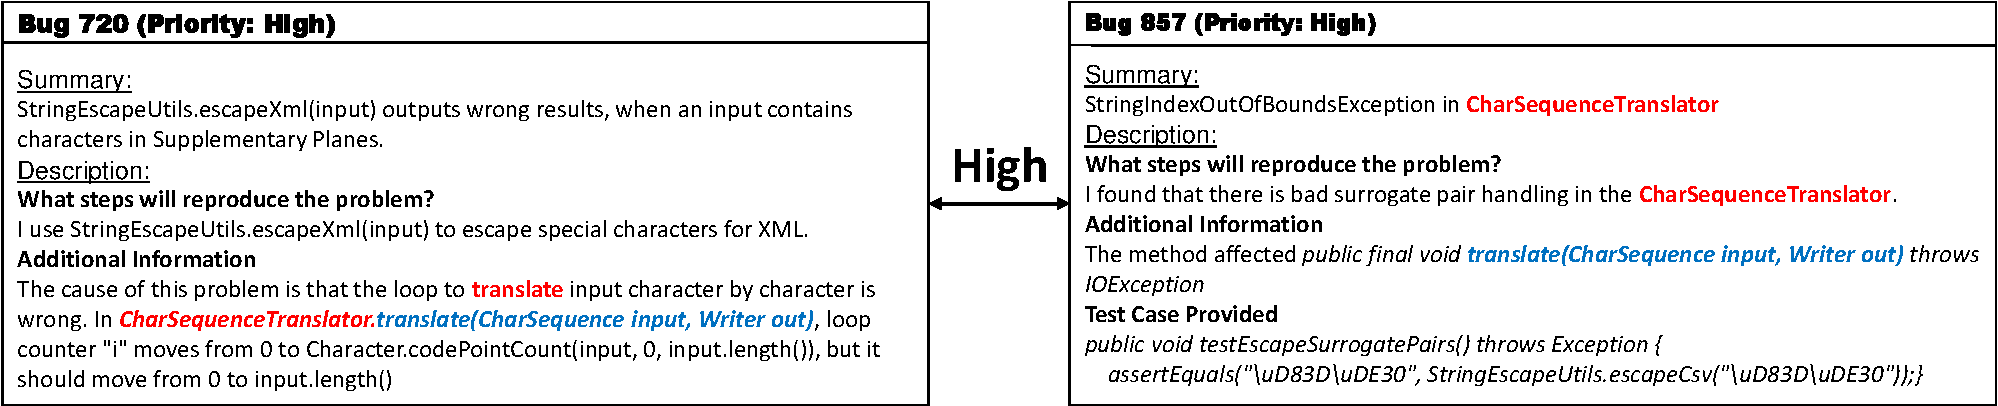
\includegraphics[width=0.55\textwidth]{bug_high_crop}
\caption{The proposed NetML framework}
\label{fig:bug_high}
\end{figure}

%\subsubsection{RQ5: Component Weights}\label{sec:rq3}
%%\begin{figure}[!htb]
%\centering
%
%\includegraphics[scale=0.5]{boxplot.eps}
%\caption{Contribution of $AML^{SPECTRA}$, $AML^{TEXT}$, and $AML^{BOTH}$}
%\label{fig:boxplot}
%\end{figure}

\begin{table}[!htb]
	\caption{Average Weights of Each Component }
	\centering
    \begin{tabular}{|c|c|c|c|}
    \hline
    \textbf{Project} & $\textbf{AML}^\textbf{Text}$ & $\textbf{AML}^{\textbf{SuspWord}}$ & $\textbf{AML}^\textbf{Spectra}$ \\ \hline\hline
AspectJ&-14.25&33.18&1.94\\\hline
Ant&9.14&12.5&1.54\\\hline
Lucene&12.43&25.77&-0.47\\\hline
Rhino&2.79&1.44&1.81\\\hline
    \end{tabular}
    \label{tab:contributions}
\end{table}

%In this research question, we investigate the contributions of $AML^{SPECTRA}$, $AML^{TEXT}$, and $AML^{BOTH}$ to the overall performance of the whole approach. We consider the default setting of $AML$, i.e., $n=20$. Figure~\ref{fig:boxplot} is the box plot showing the distribution of weights assigned to $AML^{SPECTRA}$, $AML^{TEXT}$, and $AML^{BOTH}$ which correspond to the values of $\alpha$, $\beta$, and $\gamma$ respectively. From the figure, we can note that for most bugs, all of the components are given non-zero weights. This shows that each component is important for a good number of bugs. Also, $AML^{BOTH}$ is often given higher weights than the other two components. The median weights given to $AML^{BOTH}$ and $AML^{SPECTRA}$ are the same, however the third quartile of the weights given to $AML^{BOTH}$ is much higher than the third quartile of the weights given to $AML^{SPECTRA}$. The mean of the weights given to $AML^{BOTH}$, $AML^{SPECTRA}$ and $AML^{TEXT}$ are 0.41, 0.32, and 0.27, respectively. 

%In this research question, we investigate the contribution of $\text{AML}^{\text{Text}}$, $\text{AML}^\text{SuspWord}$, and $\text{AML}^\text{Spectra}$ to the performance of AML in the context of the default setting (i.e., $n=10$). Table~\ref{tab:contributions} highlights the average weights of each AML component in the four projects.  From the Table~\ref{tab:contributions}, $\text{AML}^\text{SuspWord}$ has the highest weights than the other two components in AspectJ, Ant, and Lucene. For Rhino, $\text{AML}^\text{Text}$ has the highest weight (i.e., 2.79). Interestingly, according to Equation~\ref{eqn:composite}, component weights (i.e., $\alpha$, $\beta$, and $\gamma$) can be possible or negative numbers. From the table, AspectJ and Lucene are the two cases have negative component weights. Overall, we find that the component weights are well-tuned to maximize their contributions to the overall AML.

%[say something about the negative weights later ...]
We use default setting of AML ($n=10$) to evaluate contributions of component weights to the effectiveness of  AML. From Equation~\ref{eqn:composite}, we observe that component weights with large absolute values  have stronger influences on final suspiciousness scores of methods (i.e., $f(x_i, \theta)$), and near-zero weights have weaker influences on the suspiciousness scores. Based on our observation and the  result shown in Table~\ref{tab:contributions}, we find that average weights of AML$^\text{Text}$ and AML$^\text{SuspWord}$ in AspectJ, Ant, and Lucene are significantly larger than of AML$^\text{Spectra}$. This implies AML$^\text{Text}$ and AML$^\text{SuspWord}$ have stronger contribution to performance of AML than  AML$^\text{Spectra}$ in AspectJ, Ant, and Lucene. In Rhino, 
AML$^\text{Text}$ has the largest average weight, and AML$^\text{SuspWord}$ has the smallest weight. However, their differences are not significant compared to their magnitudes. Therefore, contributions of the three components to AML in Rhino are  relatively equivalent. On the other hand, AML$^\text{Text}$ and AML$^\text{Spectra}$ have negative average weights in AspectJ and Lucene, respectively. From Equation~\ref{eqn:composite}, we  observe that the purpose of negative weights is to decrease suspiciousness scores of methods when their magnitudes are much larger from the actual suspiciousness. Therefore, negative weights of SW$^\text{Text}$ and AML$^\text{Spectra}$ are for adjusting suspiciousness scores of methods to converge their actual values as much as possible.

%\subsection{RQ4: Adaptive vs. Non-Adaptive}\label{sec:rq4}
%%\begin{table}[t]
%	\centering
%	\caption{Adaptive vs. Non-Adaptive}
%    \begin{tabular}{|c|c|c|c|c|}
%    \hline
%      \textbf{Setting}& {\textbf{SR@1}} &\textbf{SR@5} &\textbf{SR@10} & \textbf{MAP} \\
%    \hline
%      \textbf{Adaptive} &{17.83\%}&{43.95\%}&{54.78\%}&\multirow{2}{*}{0.218}\\
%    ($AML$)   &(28)&(69)&(86)&\\\hline
%  \textbf{Non-Adaptive} &{???\%}&{???\%}&{???\%}&\multirow{2}{*}{???}\\
%	     ($AML_{*}$)  &(???)&(???)&(???)&\\\hline
%
%    
%    \end{tabular}
%    \label{tab:non_adaptive}
%\end{table}


\begin{table}[t]
	\centering
	\caption{Adaptive vs. Non-Adaptive}
	\scalebox{0.95}{
    \begin{tabular}{|c|c|c|c|c|c|}
    \hline
      \textbf{Project}& \textbf{Setting}&{\textbf{SR@1}} &\textbf{SR@5} &\textbf{SR@10} & \textbf{MAP} \\
    \hline
    \multirow{3}{*}{AspectJ} &$n=20$& 14.63\%&24.39\%&29.27\%&0.163   \\
    &$n=35$&19.51\%&26.83\%&31.71\%&0.199\\ 
    &$AML_{*}$&19.51\%&26.83\%&31.71\%&0.197\\\hline
     \multirow{3}{*}{Ant}  &$n=20$  &15.09\%&39.62\%&58.49\%&0.220 \\ 
&  $n=35$  &16.98\%&43.40\%&58.49\%&0.248\\
        &$AML_{*}$&13.21\%&41.51\%&58.49\%&0.228\\\hline
 \multirow{3}{*}{Lucene}& $n=20$ &29.73\%&64.86\%&75.68\%&0.284  \\ 
&$n=35$ &29.73\%&62.16\%&70.27\%&0.280\\
        &$AML_{*}$&29.73\%&62.16\%&70.27\%&0.280\\\hline
    \multirow{3}{*}{Rhino}&$n=20$   &11.54\%&53.85\%&57.69\%&0.204\\
    &$n=35$ &11.54\%&53.85\%&53.85\%&0.199\\
     & $AML_{*}$   &11.54\%&53.85\%&53.85\%&0.199\\\hline
    \textbf{ \multirow{3}{*}{Overall}}& $n=20$&17.83\%&43.95\%&54.78\%&0.218 \\
   
    &$n=35$ &19.75\%&45.22\%&53.50\%&0.234\\ 
      &$AML_{*}$ &18.47\%&44.59\%&53.50\%&0.227\\\hline
    \end{tabular}}
    \label{tab:non_adaptive}
\end{table}



\section{Discussion}
\label{sec:threats}

In this section, we discuss how NetML works in fault localization problem. We briefly show some examples and explain a case when NetML achieves good/poor performance. Moreover, there are several threats that may potentially impact the validity of our study. We also discuss these threats below.

\subsection{How does NetML work in Fault Localization?}
NetML contains two sets of latent parameters (i.e., bug reports and methods). The incorporation of the latent parameters provides NetML with a higher freedom to capture the relationship of different bug reports and methods more accurately. Moreover, NetML also employs the network Lasso regularization in its learning procedure, which imposes similar bug reports (and methods) to have similar latent parameters. Outputs of our NetML include the latent parameters of bug reports ($\mathbf{U}$) and methods ($\mathbf{V}$). Please refer to Section~\ref{sec:approach} for more details about NetML. 

Based on the latent parameters of bug reports (or methods), we apply cosine similarity~\cite{Salton:1975:VSM:361219.361220} to estimate how these bug reports are similar in latent space. Then we present some qualitative examples to illustrate the poor/good performance of NetML compared to other techniques. %More specifically, we show four case samples as follows:
%\begin{itemize}
%	\item A high cosine similar score of latent parameters between two bug reports. 
%	\item A low cosine similar score of latent parameters between two bug reports. 
%	\item A high cosine similar score of latent parameters between two methods. 
%	\item A low cosine similar score of latent parameters between two methods. 	
%\end{itemize}

\subsubsection{Case Examples of NetML: Good Results in Detecting Bugs}
\label{sec:case_good}
We introduce two examples defect to illustrate why NetML performs well in fault localization problem. We consider two bugs (i.e., Bug 720 and Bug 857) in project Lang. Bug 720 issues an ``outputs wrong results, when an input contains characters in \textit{Supplementary Planes}'' whereas Bug 857 contains ``\textit{StringIndexOutOfBoundsException}'' error. These two bugs ultimately reside in the \texttt{translate} method in the \texttt{CharSequenceTranslator.java} program. To find this method, based on the report, the developer could apply IR-based or spectrum-based bug localization techniques to generate a ranked list of methods. The list could then be inspected, in order, until the root cause of the bug is localized. Figure~\ref{fig:bug_high_crop} shows the description of two bugs (i.e., Bug 720 and Bug 857) in project Lang, which contains 5,528 methods. AML and SAVANT assign Bug 857 a high priority, i.e., localizing the \texttt{translate} method in the top 10 of the produced list. However, AML and SAVANT assign Bug 720 a low priority, i.e., localizing the \texttt{translate} method in the top 100 of the produced list. None of eight state-of-the-art spectrum fault localization techniques (i.e., OCHIAI, DSTAR, PROMESIR, DIT$^\text{A}$, DIT$^\text{B}$, LR$^\text{A}$, LR$^\text{B}$, and MULTRIC) localize the \texttt{translate} method within the top 10 of the produced list in both Bug 720 and Bug 857. The two best performance of spectrum fault localization approaches for this defect (i.e., OCHIAI and DSTAR) assigns the highest suspiciousness score to the faulty method; however, there are more than 100 methods sharing this score. Existing spectrum-fault localization approaches present limited utility for the developer in this case. 

On the other hand, NetML assigns Bug 720 and Bug 857 a high priority, which successfully localizes the faulty method (i.e., \texttt{translate}) within the top 10 of the produced list. Typically, we see that both NetML and AML assign Bug 857 a high priority. However, we assume that NetML takes advantages of the latent parameters of the two similar bug reports, and enforce them to have similar latent parameters. To explain our assumption, we apply a \textit{Vector Space Model} (VSM) to estimate the similarity between Bug 720 and Bug 857 at this space. We represent each bug report as vectors of weights; each weight corresponds a term. We evaluate the value of each weight by applying TF-IDF~\cite{Ramos1999} and estimate cosine similarity of Bug 857 with the remaining bug reports. We found that Bug 720 is ranked at position \textit{\#}39. We took the latent parameters of bug reports, which are the matrix $\mathbf{U}$ (please refer to Algorithm~\ref{alg:network_lasso}). We again estimate the cosine similarity of Bug 857 with the remaining bug reports in a latent space. In this case, Bug 720 is ranked at position \textit{\#}5. It shows that these two bugs are actually very close in the latent space. Indeed, these two bugs share the same \texttt{translate} method and  \texttt{CharSequenceTranslator} program, and these two bugs should be similar. AML only assumes that bug reports are independent, leading to failing to assign Bug 720 a high priority. On the other hand, NetML tries to enforce the similar bug reports to have similar latent parameters, leading to successfully to assign Bug 720 a high priority. 

Figure~\ref{fig:method_high_crop} presents the description of Bug 93 in project Time, which contains 4,181 methods. Bug 93 issues an error when ``weekyear has a null range duration type''. The bug resides in the \texttt{partial} and \texttt{compareTo} methods of the \texttt{Partial.java} and \texttt{UnsupportedDurationField.java} programs respectively. AML localizes the \texttt{partial} method in the top 5 of the produced list, however AML ranks the \texttt{compareTo} method at position \textit{\#}35. SAVANT also restricts the \texttt{partial} method in the top 10, and it ranks \texttt{compareTo} method at position \textit{\#}87. The spectrum fault localization techniques rank these two methods outside the top 100 of the produced list, which assigns this bug a low priority. NetML localizes the \texttt{partial} and \texttt{compareTo} methods at the rank \textit{\#}3 and \textit{\#}10 of the produced list respectively, which assigns Bug 93 a high priority. Similar to bug reports, we again calculate the similarity between two methods at the low space (vector space) and latent space. We collected the latent parameters of methods which are the matrix $\mathbf{V}$ (please refer to Algorithm~\ref{alg:network_lasso}). By applying VSM, we estimate cosine similarity of \texttt{partial} method with the remaining methods. We found that \texttt{compareTo} method is ranked at position \textit{\#}981. However, \texttt{compareTo} method is ranked at position \textit{\#}32 in the latent space. By looking at the content of these two methods, we see that they share the same parameter \texttt{DurationField} and \texttt{compareTo}, hence these methods should be close. AML assumes that methods are independent, leading to failing to localize the faulty \texttt{compareTo} method. NetML enforces the similar methods to have highly similar latent parameters, leading to successfully to localize \texttt{compareTo} method at rank \textit{\#}10. 

\subsubsection{Case Examples of NetML: Poor Results in Detecting Bugs}
\label{sec:case_bad}
We first introduce two examples defect to show why NetML achieves poor performance in fault localization problem. We consider Bug 617 and Bug 710 in project Lang. Bug 617 contains an error of ``process UTF-16 supplementary characters'' whereas Bug 710 has ``StringIndexOutOfBoundsException'' when we call a special string. These two bugs are related the \texttt{escapeXML} method in the \texttt{StringEscapeUtils.java} program. Figure~\ref{fig:bug_low} presents the details of these two bugs. NetML, AML, and SAVANT assign Bug 617 a high priority, however they fail to localize the faulty \texttt{escapeXML} method for Bug 710. Intuitively, \texttt{escapeXML} method and \texttt{StringEscapeUtils} program were clearly mentioned in Bug 617, hence should be easily captured by applying IR-based localization technique. OCHIAI and DSTAR estimate the highest suspiciousness score to the \texttt{escapeXML} method for both Bug 617 and Bug 710; however, we have around 50 methods sharing this score. The remaining baselines (i.e., PROMESIR, DIT$^\text{A}$, DIT$^\text{B}$, LR$^\text{A}$, LR$^\text{B}$, and MULTRIC) fail to localize these two bugs in a high priority. By reading the content of Bug 710, we see that this bug does not contain any information related to \texttt{escapeXML} method. Moreover, the suspiciousness score of the faulty method, which is calculated by using spectrum-fault localization, often shares with another methods. For these reasons, it is a challenge to assign a high priority for Bug 710. Similar to Section~\ref{sec:case_good}, we calculate the similarity score between these two bugs at low and latent spaces. We estimate the similarity of Bug 617 with the remaining bug reports. We found that Bug 710 is ranked at position \textit{\#}55 and \textit{\#}48 in the low level space and latent space, respectively. It shows that these two bugs are independently, and hence NetML fails to localize the faulty method for bug 710.

Figure~\ref{fig:method_low} shows the descriptions of Bug 18 in project Time. Bug 18 issues an null pointer exception when ``a DateTimeZone is build with duplicate-named''. The bug contains two faulty methods, i.e., \texttt{RuleSet} and \texttt{DateTimeOfYear}, in \texttt{ZoneInfoCompiler.java} program. NetML, AML, and SAVANT localizes the \texttt{RuleSet} method in the top 10 of produced list, however these techniques rank \texttt{DateTimeOfYear} method outside the top 50. OCHIAI and DSTAR rank these methods at the highest suspiciousness score, however we have 42 methods sharing this score. The other baselines fail to localize the two faulty methods within the top 50 of the produced list. We again estimate the similarity score between the two methods at a low level space and latent space. We calculate the similarity of method \texttt{RuleSet} against the remaining methods in Time. Method \texttt{DateTimeOfYear} is ranked at position \textit{\#} 2,678 and \textit{\#}2,468 in the low level space and latent space, respectively. It shows that these two methods independent with each other, hence NetML is unable to localize method \texttt{DateTimeOfYear}.

%\begin{figure*}[!t]
%	\centering
%	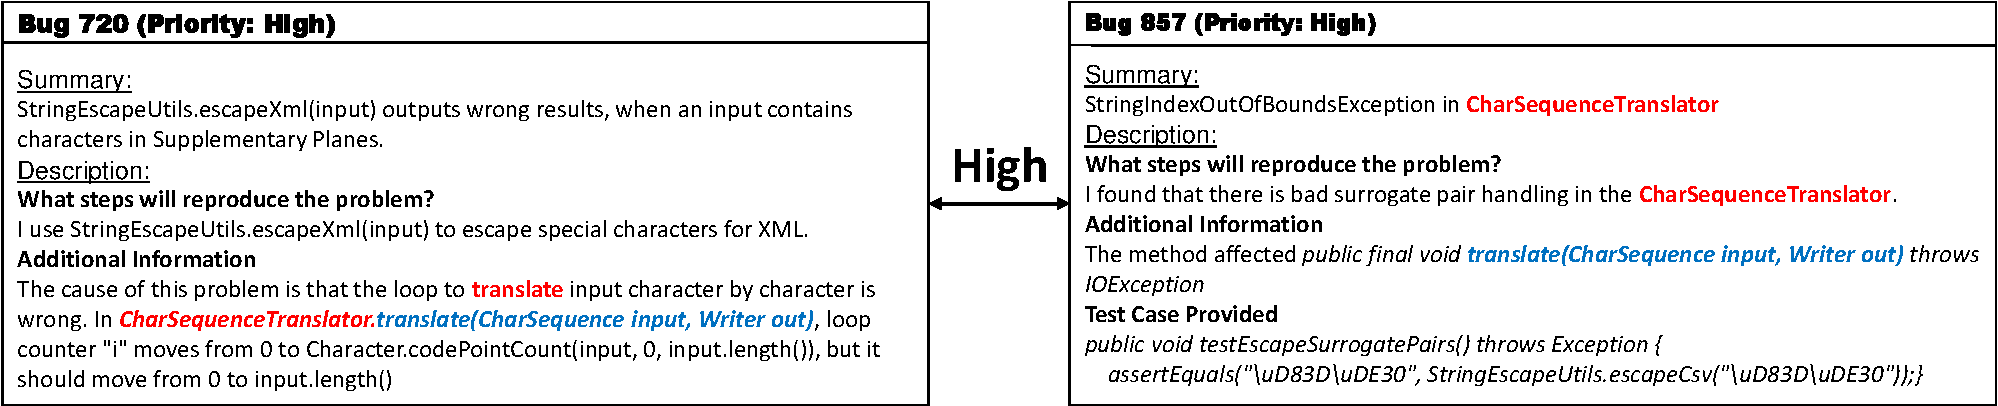
\includegraphics[width=\textwidth]{bug_high_crop}
%	\caption{The proposed NetML framework}
%	\label{fig:bug_high_crop}
%\end{figure*}

\begin{figure*}
	\centering
	\begin{subfigure}[b]{\textwidth}
		\centering
		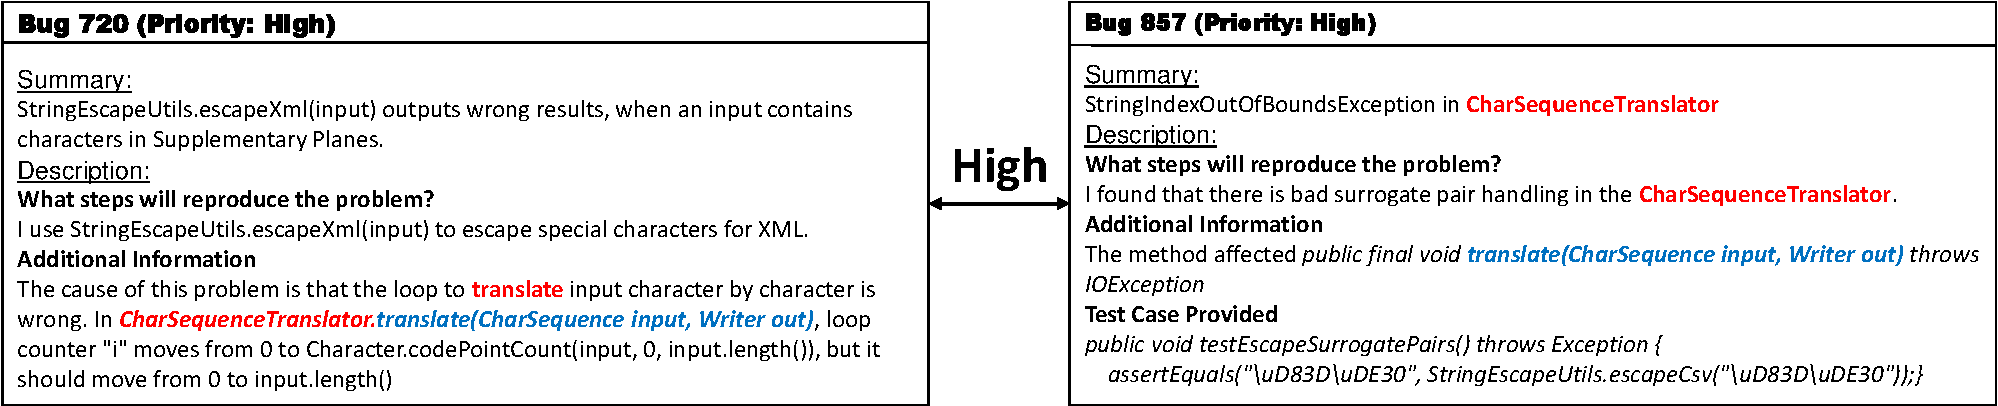
\includegraphics[width=\textwidth]{bug_high_crop}
		\caption[]%
		{{\small A case example which NetML achieves a good results. Two bug reports are highly similar at latent space.}}    
		\label{fig:bug_high_crop}
	\end{subfigure}
	\centering
	\begin{subfigure}[b]{\textwidth}  
		\centering 
		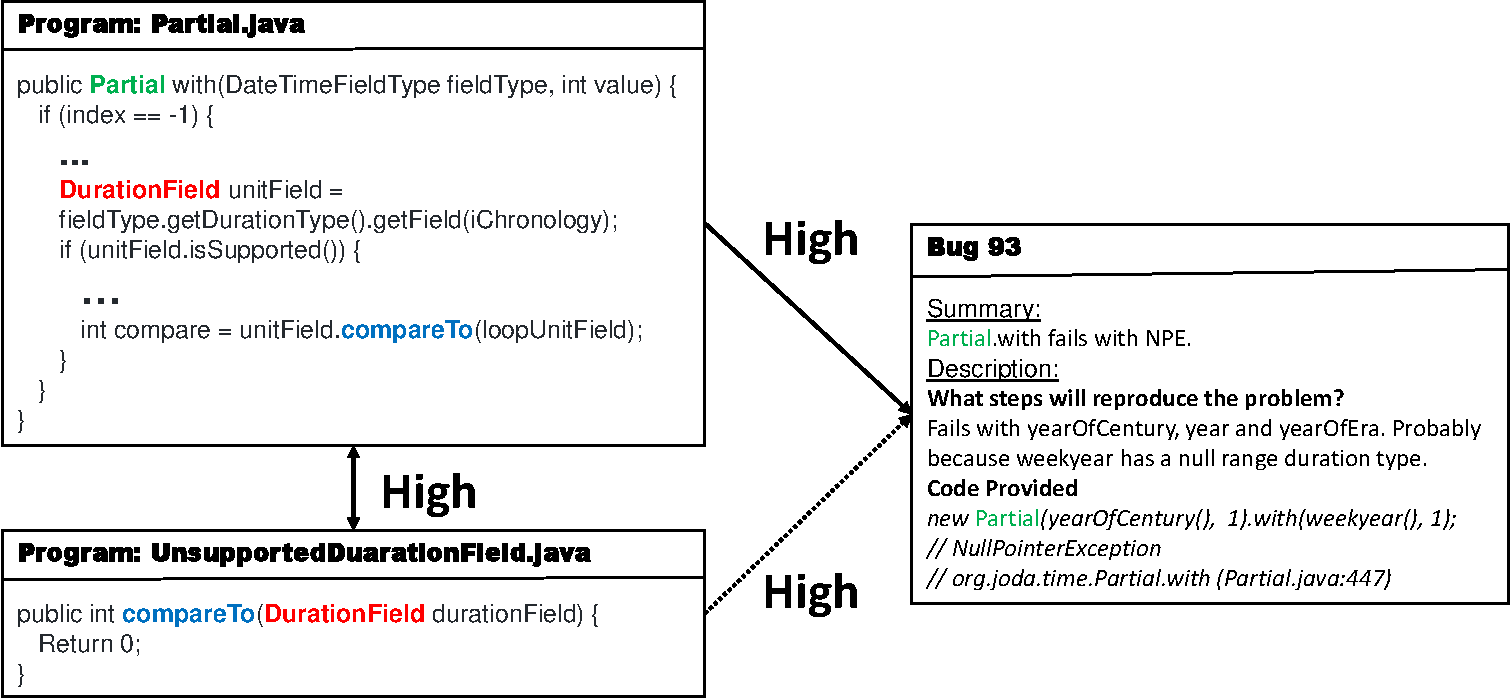
\includegraphics[width=\textwidth]{method_high_crop.pdf}
		\caption[]%
		{{\small A case example which NetML achieves a good results. Two methods are highly similar at latent space.}}    
		\label{fig:method_high_crop}
	\end{subfigure}
	\caption[]
	{\small A list of case examples to illustrate why NetML achieves good performance.}
\label{fig:case_good_example}

\end{figure*}
\begin{figure*}
	\centering
	\begin{subfigure}[b]{\textwidth}
		\centering
		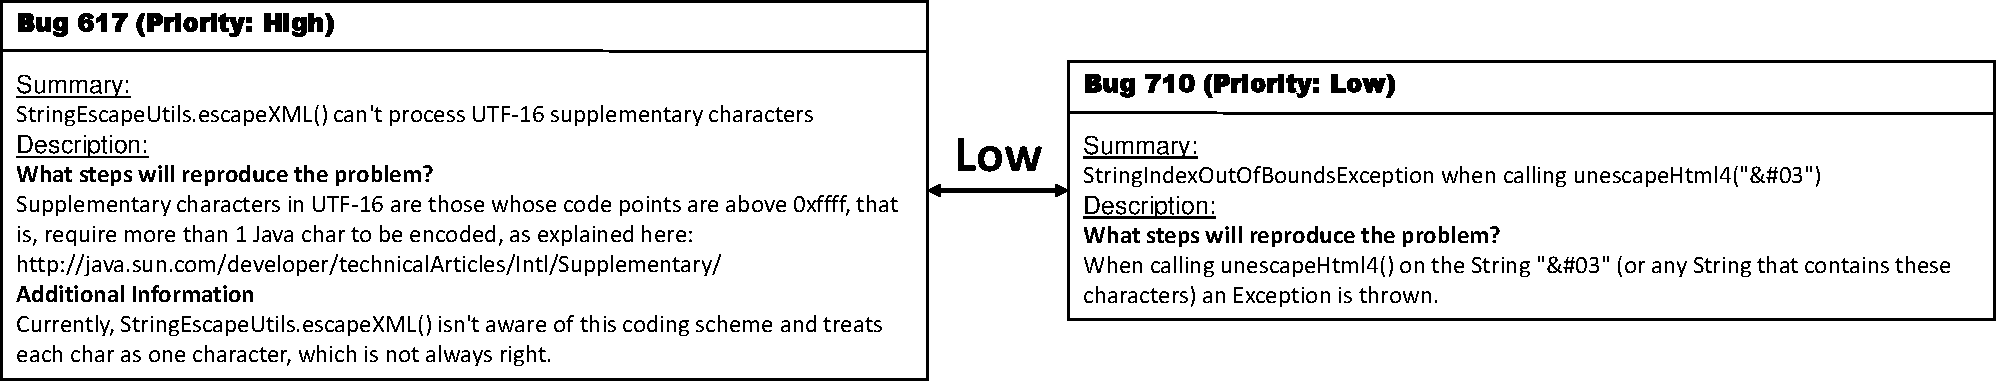
\includegraphics[width=\textwidth]{bug_low}
		\caption[]%
		{{\small A case example which NetML achieves a bad results. Two bug reports has a low similar at latent space.}}    
		\label{fig:bug_low}
	\end{subfigure}
	\centering
	\begin{subfigure}[b]{\textwidth}  
		\centering 
		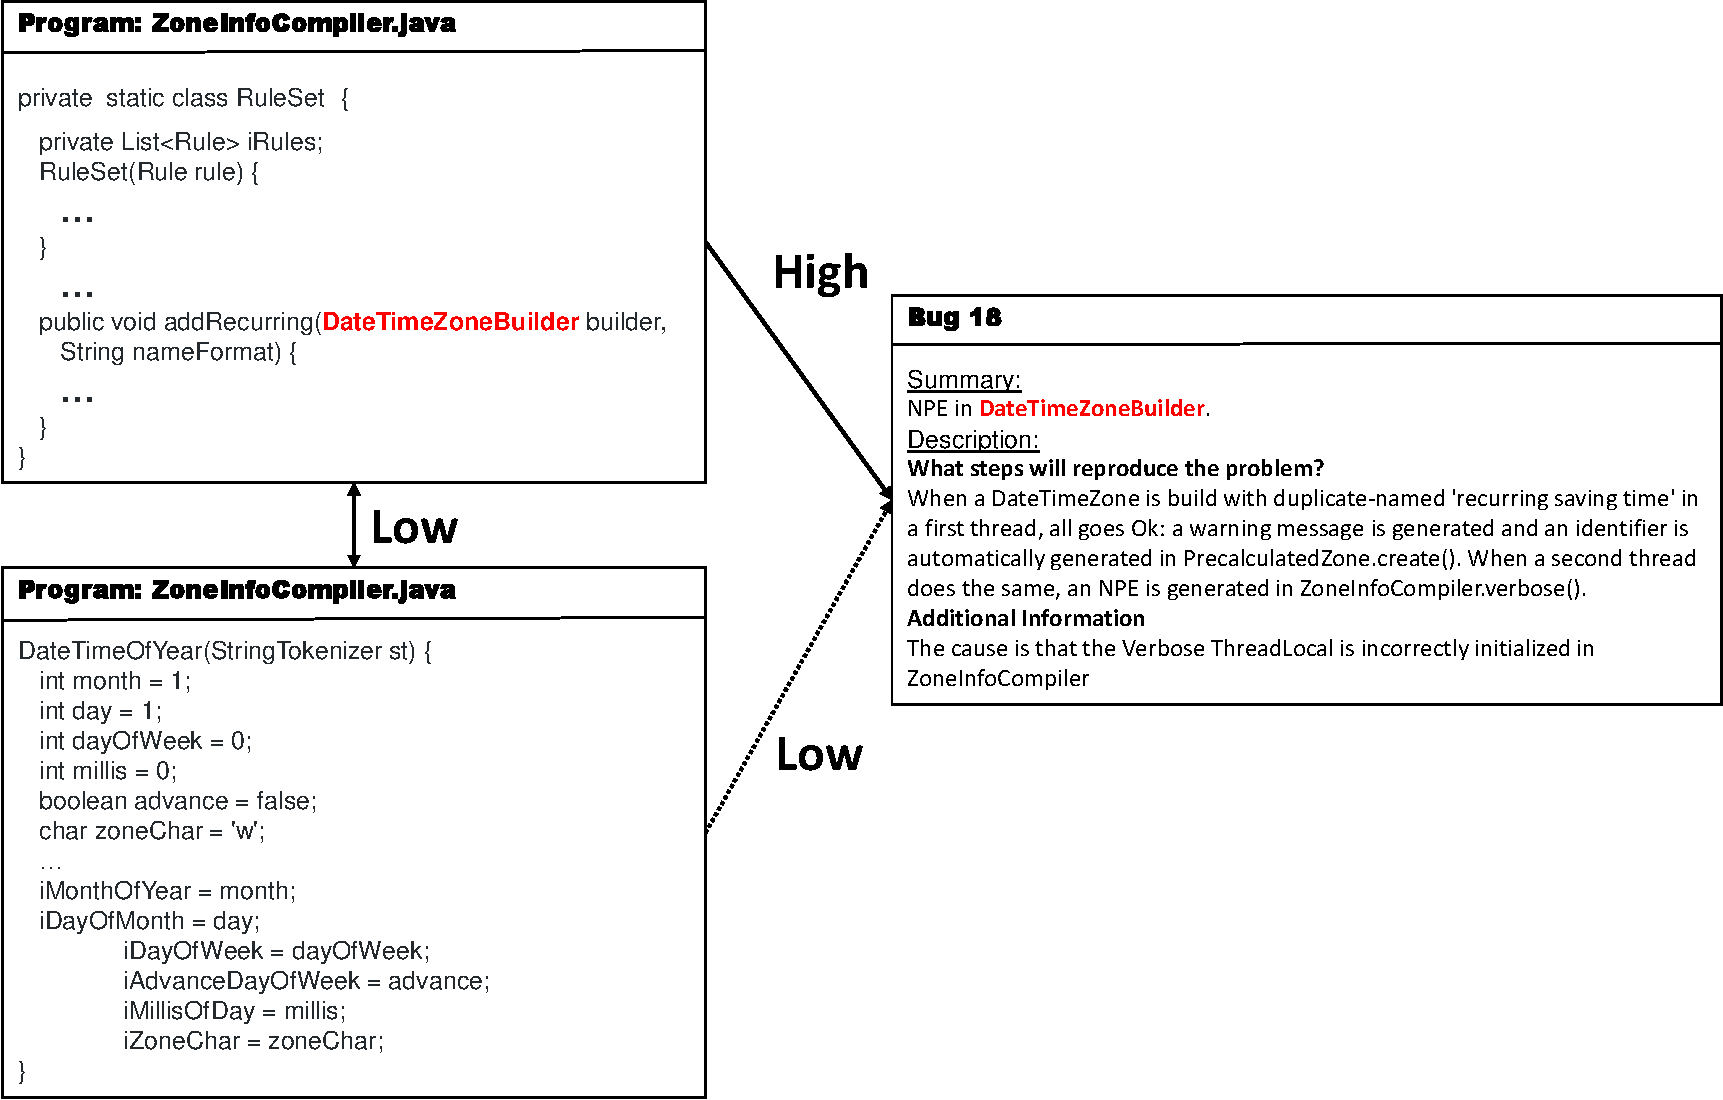
\includegraphics[width=\textwidth]{method_low_crop.pdf}
		\caption[]%
		{{\small A case example which NetML achieves a bad results. Two methods has a low similar at latent space.}}    
		\label{fig:method_low}
	\end{subfigure}
	\caption[]
	{\small A list of bad case examples to illustrate why NetML achievespoor performance.} 
	\label{fig:case_bad_example}
\end{figure*}





\subsection{Number of Failed Test Cases and Its Impact}

In our experiments with 157 bugs, most of the bugs were found to come with few failed test cases (average = 2.185). We have investigated if the number of failed test cases impacts the effectiveness of our approach. To this end, we computed the differences between the average number of failed test cases for bugs that are successfully localized at top-N positions (N = 1,5,10) and bugs that are not successfully localized. We found that the differences are small (-0.472 to 0.074 test cases). These indicate that the number of test cases does not impact the effectiveness of our approach significantly and typically 1 to 3 failed test cases are sufficient for our approach to be effective.

\subsection{Threats to Internal Validity} 

Threats to internal validity relate to implementation and dataset errors. We have checked our implementations and datasets. However, there could still be errors that we do not notice. Threats to external validity relate to the generalizability of our findings. In this work, we have analyzed 157 real bugs from 4 medium-large software systems. In the future, we plan to reduce the threats to external validity by investigating more real bugs from additional software systems, written in various programming languages. 

%\subsubsection{Threats to Construct Validity}
%
%Threats to construct validity relate to the suitability of our evaluation metrics and experimental settings. Both Top N and MAP have been used to evaluate many past bug localization studies~\cite{Rao:2011:RSL:1985441.1985451,Sisman:2012:IVH:2664446.2664454,Zhou:2012:BFM:2337223.2337226,SahaLKP13}. MAP is also well known in the information retrieval community~\cite{Manning2008}. We have performed cross validation to evaluate the effectiveness of approach on various training and test data. Cross validation is a standard setting used to evaluate many past studies~\cite{Anvik:2006:FTB:1134285.1134336,HooimeijerW07,DAmbrosLR10,ShivajiWAK13}. Unfortunately, cross validation ignores temporal ordering among bug reports. If bugs reported at different dates do not exhibit substantially different characteristics in terms of their program spectra and descriptions, then this threat is minimal.

%The creation of our datasets follow the heuristics described by Dallmeier and Zimmermann~\cite{DallmeierZ07}. These heuristics are not guaranteed to be perfect; for example, there could be some bug fixing commits that are not linked to their corresponding bug report. Still, all these systems are written in Java and open source. We also plan to investigate the effectiveness of our bug localization technique on closed-source or industrial software systems.
 
%Thus, we believe there is little threat to construct validity from evaluation metrics.

%Thus, we believe it is reasonable to ignore temporal ordering. In the future, we plan to evaluate our approach in different settings that captures date information of bug reports. \color{red}In addition to textual descriptions, bug reports contain date information (i.e., report dates) in their contents. These information can be used to construct a temporal order between bug reports. However, until now, it is unclear whether ordering of bug reports have impacts on root causes of bugs. For example, \textit{Null Pointer Exception} can happen anytime regardless the occurrences of  other bugs.}
